\documentclass[13pt]{report}
\usepackage[utf8]{vietnam}
\usepackage[paperheight=29.7cm,paperwidth=21cm,right=2cm,left=3cm,top=2.5cm,bottom=2.5cm]{geometry}
\usepackage[table,xcdraw]{xcolor}
\usepackage{indentfirst}
\usepackage{graphicx}
\usepackage{titlesec}
\usepackage{amsmath}
\setlength{\parindent}{4cm}
\renewcommand{\baselinestretch}{1.2}
\renewcommand\thesection{\arabic{section}}
\setlength{\parskip}{0.3pt}
\setlength{\parindent}{0.5cm}
\usepackage{fancyhdr}
\pagestyle{fancy}
\lhead{\textbf{Triển khai, Quản lý, Cấu hình Certificate Services}}
\chead{}
\rhead{\textbf{\textit{Quản trị hệ thống mạng}}}
\lfoot{\textbf{Giảng viên: Lê Viết Thanh}}
\cfoot{}
\rfoot{\thepage}
\renewcommand{\headrulewidth}{0.4pt}
\renewcommand{\footrulewidth}{0.4pt}
\allowdisplaybreaks
\titleformat{\section}{\normalfont\huge\bfseries}{\thesection}{1em}{}
\titleformat{\subsection}{\normalfont\LARGE\bfseries}{\thesubsection}{1em}{}
\titleformat{\subsubsection}{\normalfont\LARGE\bfseries}{\thesubsection}{1em}{}
\usepackage{caption}
\captionsetup[figure]{font=large}
\begin{document}
	\pagenumbering{gobble}
	\fontsize{14pt}{20pt}\selectfont
	\begin{center}
		BỘ GIÁO DỤC VÀ ĐÀO TẠO\\
		\textbf{TRƯỜNG ĐẠI HỌC TÔN ĐỨC THẮNG}\\
		\textbf{KHOA CÔNG NGHỆ THÔNG TIN} \\
		\vspace*{1cm}
	\end{center}
	\begin{figure}[h]
		\centering
		\includegraphics[width=0.5\linewidth]{image/logo.png}\\\vspace*{1cm}	
	\end{figure}
	\fontsize{20pt}{20pt}\selectfont
	\begin{center}
		\textbf{QUẢN TRỊ HỆ THỐNG MẠNG}
	\end{center}
	\vspace{2cm}
	\fontsize{16pt}{20pt}\selectfont
	\begin{flushright}			
		\textit{Người thực hiện:} \\
		\textbf{Nguyễn Dư Thành Long - 52100976}\\
		\textbf{Đinh Phương My - 52100703}\\
		\textbf{Đặng Minh Phong - 52100987}\\\vspace{0.5cm}
		\textit{Nhóm:}
		\textbf{20}\\\vspace{0.5cm}
		\textit{Giảng viên hướng dẫn:} \\
		\textbf{Lê Viết Thanh}
	\end{flushright}
	\vspace{2cm}
	\fontsize{16pt}{20pt}
	\begin{center}
		\textbf{THÀNH PHỐ HỒ CHÍ MINH – 2023}
	\end{center}
	\newpage
	\pagestyle{fancy}
	\lhead{\textbf{Triển khai, Quản lý, Cấu hình Certificate Services}}
	\chead{}
	\rhead{\textbf{\textit{Quản trị hệ thống mạng}}}
	\lfoot{\textbf{Giảng viên: Lê Viết Thanh}}
	\newpage
	\pagenumbering{arabic}
	\setcounter{page}{1}
	\newpage
	\begin{center}
		\textbf{LỜI CẢM ƠN}
	\end{center}
	Nhóm 20 xin được gửi lời cảm ơn đến thầy Lê Viết Thanh đã tận tình giảng dạy và giúp đỡ nhóm trong việc hoàn thành bài tập, cũng như hiểu vấn đề của môn học đề ra.\\
	Với những kiến thức nhóm 20 tích lũy được qua những ngày học tập, đây là kết quả của quá trình học tập của nhóm. Tuy vẫn còn nhiều mặt còn hạn chế, nhưng nhóm 20 sẽ cố gắng để đạt được kết quả tốt nhất có thể.\\
	\newpage
	\begin{center}
		\textbf{ĐỒ ÁN CUỐI KỲ ĐƯỢC HOÀN THÀNH} \\
		\textbf{TẠI TRƯỜNG ĐẠI HỌC TÔN ĐỨC THẮNG} \\
	\end{center}	
	Nhóm 20 xin cam đoan đây là bài báo cáo sản phẩm đồ án cuối kỳ chỉ của riêng nhóm. Các nội dung nghiên cứu, kết quả trong đề tài này là trung thực và chưa được công bố dưới bất kỳ hình thức nào. Những số liệu trong các bảng biểu phục vụ cho việc phân tích, nhận xét, đánh giá được chính tác giả thu thập từ các nguồn khác nhau có ghi rõ trong phần tài liệu tham khảo.\\
	Ngoài ra, trong đề tài còn sử dụng một số nhận xét, đánh giá cũng như số liệu của các tác giả khác, cơ quan tổ chức khác đều có trích dẫn và chú thích nguồn gốc rõ ràng và cụ thể.\\
	Nếu phát hiện có bất kỳ sự gian lận nào nhóm 20 xin hoàn toàn chịu trách nhiệm về nội dung của bài đồ án cuối kỳ  Trường đại học Tôn Đức Thắng không liên quan đến những vi phạm tác quyền trong quá trình thực hiện của em.\\
	\begin{center}
		\hspace*{5cm}TP. Hồ Chí Minh, ngày 30 tháng 11 năm 2023\\
		\hspace*{7cm}Sinh viên thực hiện,\\\vspace*{0.2cm}
		\hspace*{7cm}\textit{Nguyễn Dư Thành Long}\\
		\hspace*{7cm}\textit{Đinh Phương My}\\
		\hspace*{7cm}\textit{Đặng Minh Phong}\\
	\end{center}		
	\newpage
	\begin{center}
		\textbf{PHẦN XÁC NHẬN VÀ ĐÁNH GIÁ}
	\end{center}
	\textbf{Phần đánh giá của giảng viên chấm bài:}\\
	................................................................................................................\\
	................................................................................................................\\
	................................................................................................................\\
	................................................................................................................\\
	................................................................................................................\\
	................................................................................................................\\
	................................................................................................................\\
	\begin{center}
		\hspace*{5cm} TP. Hồ Chí Minh, ngày..... tháng..... năm 2023\\
		\hspace*{5cm} Giảng viên chấm bài,
		\vspace*{2cm}
	\end{center}
	\textbf{Phần đánh giá của giảng viên hướng dẫn:}\\
	................................................................................................................\\
	................................................................................................................\\
	................................................................................................................\\
	................................................................................................................\\
	................................................................................................................\\
	................................................................................................................\\
	................................................................................................................\\
	\begin{center}
		\hspace*{5cm} TP. Hồ Chí Minh, ngày..... tháng..... năm 2023\\
		\hspace*{5cm} Giảng viên hướng dẫn,
		\newpage
	\end{center}
	\newpage
	\tableofcontents
	\newpage
	\chapter{Lý thuyết}
	\section{Các khái niệm}
	\begin{itemize}
		\item Certificate Services (Dịch vụ chứng chỉ): Là một dịch vụ trong hệ thống Public Key Infrastructure (PKI) được sử dụng để quản lý và cấp phát chứng chỉ số (digital certificates). Chứng chỉ số đóng vai trò quan trọng trong việc xác thực và bảo mật thông tin trong các môi trường mạng, tạo điều kiện cho việc sử dụng khóa công cộng và khóa riêng tư.
		\item Public Key Infrastructure (PKI): Là một hệ thống bao gồm phần cứng, phần mềm, con người, chính sách và thủ tục, tất cả nhằm mục đích tạo, quản lý, phân phối, sử dụng, lưu trữ và thu hồi các chứng chỉ số (digital certificates). Được sử dụng để đảm bảo tính bảo mật, xác thực và toàn vẹn của thông tin trong quá trình truyền thông.
		\item Digital Certificates (Chứng chỉ số):  Là một thành phần quan trọng của PKI, chứng chỉ số là một loại tài liệu số được ký bởi một Certificate Authority (CA) để xác nhận danh tính của một đối tượng (người dùng, máy tính, hay thiết bị) và kèm theo khóa public của họ. Mục đích chính của digital certificates là thực hiện các nhiệm vụ bảo mật như xác thực, mã hóa và giữ tính toàn vẹn của dữ liệu trong một môi trường mạng.
		\item Certificate Authority (CA - Tổ chức chứng chỉ): Là một tổ chức tin cậy có trách nhiệm quản lý quá trình cấp phát chứng chỉ số. CA ký chứng chỉ số bằng cách sử dụng khóa riêng tư của mình, cung cấp chứng minh về tính hợp lệ và tin cậy của chứng chỉ.
	\end{itemize}
	\section{Tính năng}
	\begin{itemize}
		\item Cấp phát chứng chỉ
		\begin{itemize}
			\item Cho phép cấp phát chứng chỉ số cho người dùng, máy client, và máy chủ.		
			\item Hỗ trợ việc xác định và chứng thực danh tính của các thực thể trong mạng.
		\end{itemize}	
		\item Thu hồi chứng chỉ
		\begin{itemize}
			\item Hỗ trợ quá trình thu hồi chứng chỉ khi chúng không còn hợp lệ.
			\item Đảm bảo tính an toàn và tin cậy bằng cách ngăn chặn sử dụng chứng chỉ đã bị thu hồi.
		\end{itemize}	
		\item Sử dụng các Certificate Authorities (CAs)
		\begin{itemize}
			\item Sử dụng Certificate Authorities để xác thực tính hợp lệ của người dùng và máy tính.
			\item Cung cấp chứng chỉ số để chứng minh tính xác thực đó.
		\end{itemize}	
	\end{itemize}
	\section{Cách thức hoạt động}
	\begin{itemize}
		\item Yêu cầu chứng chỉ (Certificate Request)
		\begin{itemize}
			\item Người dùng, máy tính hoặc dịch vụ muốn có một chứng chỉ số để xác nhận danh tính.
			\item Một yêu cầu chứng chỉ được tạo, chứa thông tin về thực thể yêu cầu chứng chỉ và thuật toán mã hóa sẽ được sử dụng.
		\end{itemize}	
		\item Gửi yêu cầu đến Certificate Authority (CA): yêu cầu chứng chỉ được gửi đến CA, nơi quyết định liệu yêu cầu này có hợp lệ không.
		\item Xác nhận và xác định quyền (Validation and Authorization)
		\begin{itemize}
			\item CA kiểm tra xem yêu cầu có đáp ứng các tiêu chí an toàn và chính xác không.
			\item Nếu yêu cầu được chấp nhận, CA xác định quyền hạn cụ thể cho chứng chỉ (ví dụ: thời gian hiệu lực, mục đích sử dụng).
		\end{itemize}	
		\item Tạo chứng chỉ (Certificate Issuance): CA tạo một chứng chỉ mới với thông tin được xác nhận và quyền hạn được xác định.
		\item Phân phối chứng chỉ (Certificate Distribution)
		\begin{itemize}
			\item Chứng chỉ mới được gửi trở lại cho thực thể yêu cầu (người dùng, máy tính hoặc dịch vụ).
			\item Phương tiện phân phối có thể bao gồm truyền qua mạng, lưu trữ tại nơi nào đó trên mạng, hoặc thậm chí trên một thiết bị vật lý như thẻ thông minh.
		\end{itemize}	
		\item Kiểm tra chuỗi chứng chỉ (Certificate Chain Validation): Thực thể sử dụng chứng chỉ phải kiểm tra chuỗi chứng chỉ để đảm bảo rằng chứng chỉ được ký bởi một CA tin cậy và không bị thu hồi.
		\item Quản lý chuỗi chứng chỉ (CRL Management): CA duy trì một danh sách chứng chỉ bị thu hồi (CRL), và thực thể sử dụng chứng chỉ kiểm tra xem chứng chỉ có hiệu lực hay không dựa trên CRL.
		\item Tự động hóa và theo dõi (Automation and Logging)
		\begin{itemize}
			\item Các quy trình này thường được tự động hóa để giảm công việc quản trị.
			\item Sự kiện và hoạt động liên quan đến chứng chỉ thường được ghi lại để giúp theo dõi và phân tích.
		\end{itemize}	
	\end{itemize}
	\section{Tầm quan trọng}
	\begin{itemize}
		\item Bảo mật thông tin và tài nguyên: AD CS cung cấp cơ sở hạ tầng chứng chỉ để xác nhận danh tính và bảo vệ thông tin quan trọng trong môi trường doanh nghiệp. Việc sử dụng chứng chỉ giúp ngăn chặn các tấn công giả mạo và đảm bảo an toàn cho dữ liệu quan trọng.
		\item Quản lý truy cập và quyền hạn:
		Chứng chỉ được sử dụng để xác định quyền hạn và truy cập đối với người dùng, máy tính và dịch vụ trong hệ thống. Điều này giúp quản trị viên kiểm soát chính xác ai có quyền truy cập vào tài nguyên nào.
		\item Tuân thủ chuẩn mạng và an toàn:
		AD CS hỗ trợ các tiêu chuẩn chứng chỉ như X.509, giúp đảm bảo rằng hệ thống tuân thủ các chuẩn mạng và an toàn quốc tế.
		\item Tự động hóa và giảm công việc quản trị:
		Quy trình tự động hóa cấp và phân phối chứng chỉ giúp giảm công việc quản trị. Autoenrollment cho phép tự động cấp chứng chỉ cho người dùng và máy tính mà không cần sự can thiệp thủ công nhiều.
		\item Quản lý chuỗi chứng chỉ và thu hồi chứng chỉ:
		AD CS giữ cho danh sách chứng chỉ bị thu hồi (CRL) được cập nhật để ngăn chặn việc sử dụng chứng chỉ đã bị thu hồi. Điều này đóng vai trò quan trọng trong việc duy trì tính toàn vẹn và an toàn của hệ thống.
		\item Hỗ trợ mô hình chứng chỉ tùy chỉnh:
		AD CS cho phép quản trị viên tạo và quản lý các mô hình chứng chỉ tùy chỉnh, giúp đáp ứng đối với các yêu cầu cụ thể của doanh nghiệp.
		\item Hỗ trợ cho Elliptic Curve Cryptography (ECC):
		ECC là một thuật toán mã hóa mạnh mẽ với kích thước chìa khóa nhỏ hơn so với RSA. AD CS hỗ trợ ECC, cung cấp tính linh hoạt và bảo mật cao hơn.
		\item Quản lý tích hợp với Active Directory:
		AD CS tích hợp chặt chẽ với Active Directory, giúp quản trị viên quản lý chứng chỉ và quyền hạn một cách hiệu quả trong môi trường Active Directory.
	\end{itemize}
	\newpage
	\chapter{Thực hành}
	\section{Nội dung}
	\begin{itemize}
		\item \textbf{Yêu cầu:} Sử dụng Active Directory Certificate Services (ADCS) để bảo mật WebServer.
		\item \textbf{Mô hình mạng}
		\begin{figure}[htp]
			\centering
			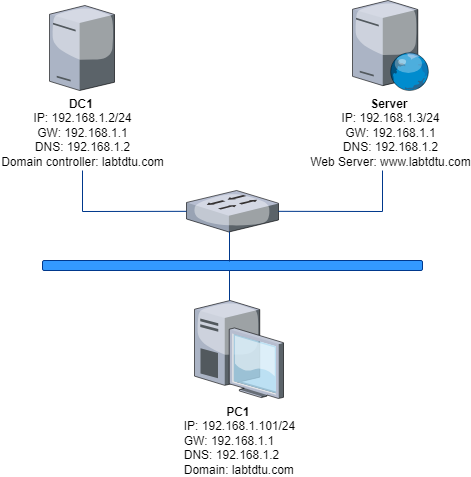
\includegraphics[width=0.7\textwidth]{image/mohinh.png}
			\caption{Mô hình mạng}
			\label{refhinh1}
		\end{figure}
		\item \textbf{Chuẩn bị}
		\begin{itemize}
			\item 2 máy Windows Server 2022 đặt tên lần lượt là DC1 và Server
			\item 1 máy Windows 8.1 Enterprise đặt tên là PC1.
		\end{itemize}
		\item \textbf{Các bước thực hiện}
		\begin{itemize}
			\item Trên máy DC1, cài đặt Active Directory Domain Controller. Sau đó join máy Server vào domain và PC1 vào domain
			\item Trên máy Server, cài đặt Active Directory Certificate Services và cấu hình Web Server.
			\item Đứng trên máy PC1 truy cập vào web site: www.labtdtu.com
			\item \textbf{Chú ý:} Khi thực hiện trên GUI thì các tên máy không đổi nhưng khi thực hiện trên PowerShell các tên sẽ có một chút thay đổi để không bị lẫn lộn, các tên được thay đổi như sau:
			\begin{itemize}
				\item DC1 đổi thành FIT-DC
				\item Server đổi thành FIT-WEB
				\item PC1 đổi thành FIT-WIN08-01
			\end{itemize}
		\end{itemize}
	\end{itemize}
	\newpage
	\section{Thực hành trên GUI}
	\subsection{Cài đặt Active Directory Domain}
	\begin{itemize}
		\item Trên máy DC1, cài đặt địa chỉ IP tĩnh cho server trước khi thực hiện cài đặt	
		\begin{figure}[htp]
			\centering
			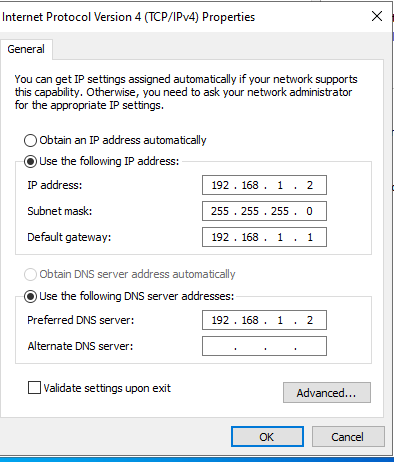
\includegraphics[width=0.7\textwidth]{image/Gui/ADDC/0.png}	
			\caption{Thiết lập ip cho Domain Controller}
			\label{refhinh1}
		\end{figure}
		\item Chọn menu Start > Administrative Tools > Server Manager. Chọn Roles > Add Roles and Features
		\newpage
		\item Xuất hiện cửa sổ Before You Begin, chọn Next.
		\begin{figure}[htp]
			\centering
			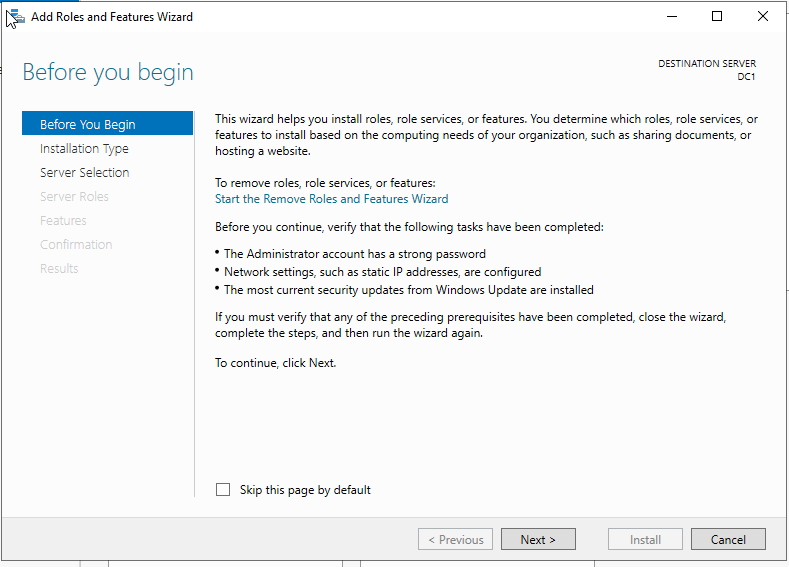
\includegraphics[width=0.72\textwidth]{image/Gui/ADDC/2.png}
			\caption{Cửa sổ Before You Begin}
			\label{refhinh1}
		\end{figure}
		\item Xuất hiện cửa sổ Select Installation Type, chọn Role-based or feature-based installation > Next
		\begin{figure}[htp]
			\centering
			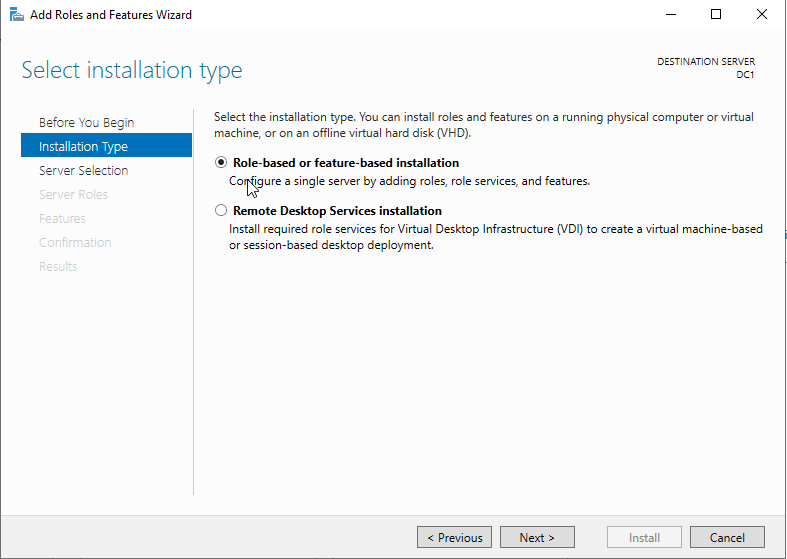
\includegraphics[width=0.72\textwidth]{image/Gui/ADDC/3.png}
			\caption{Thiết lập ip cho Domain Controller}
			\label{refhinh1}
		\end{figure}
		\newpage
		\item Xuất hiện cửa sổ Select Destination Server, chọn Select a server from the server pool > Next
		\begin{figure}[htp]
			\centering
			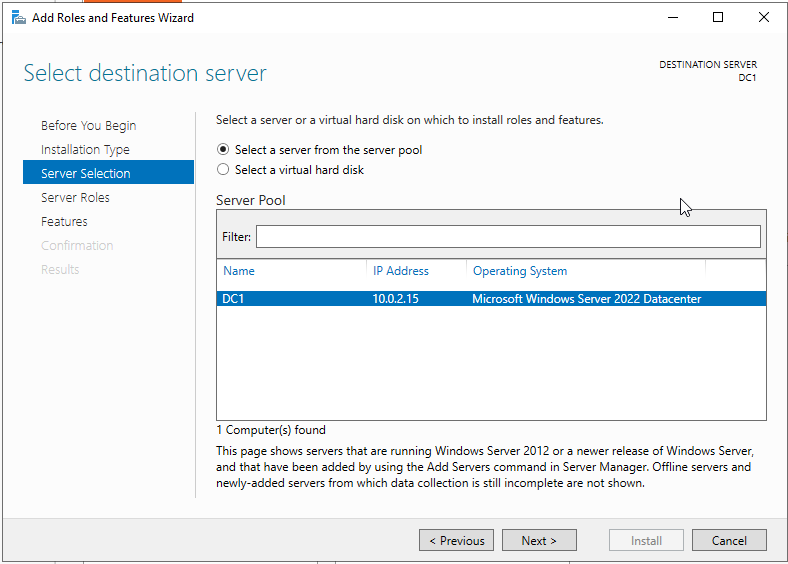
\includegraphics[width=0.7\textwidth]{image/Gui/ADDC/4.png}
			\caption{Cửa sổ Select Destination Server}
		\end{figure}
		\item Xuất hiện cửa sổ Select Server Roles, chọn mục Active Directory Domain Services > Next
		\begin{figure}[htp]
			\centering
			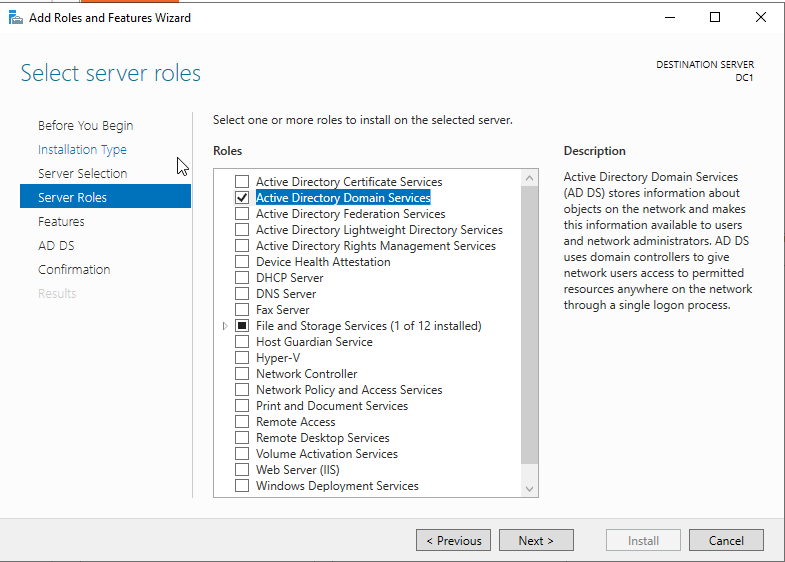
\includegraphics[width=0.7\textwidth]{image/Gui/ADDC/5.png}
			\caption{Cửa sổ Select Server Roles}
		\end{figure}
		\newpage
		\item Các tính năng bổ sung được yêu cầu để thêm AD DS. Nhấp vào nút Add Features.
		\begin{figure}[htp]
			\centering
			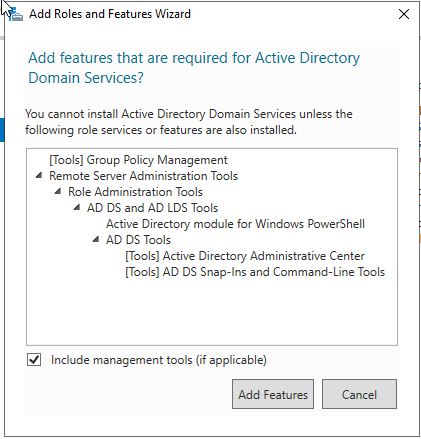
\includegraphics[width=0.5\textwidth]{image/Gui/ADDC/6.png}
			\caption{Các tính năng bổ sung}
		\end{figure}
		\item Xuất hiện cửa sổ Select Features, chọn Next.
		\begin{figure}[htp]
			\centering
			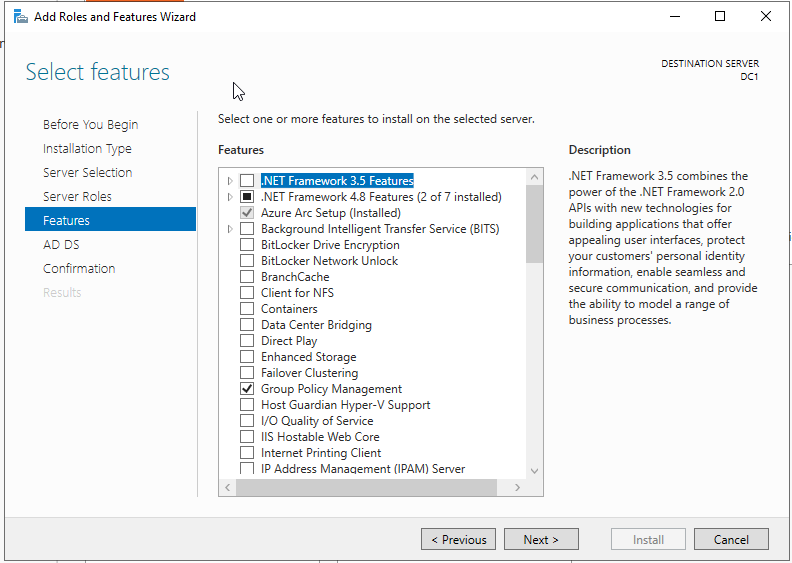
\includegraphics[width=0.7\textwidth]{image/Gui/ADDC/7.png}
			\caption{Cửa sổ Select Features}
		\end{figure}
		\newpage
		\item Xuất hiện cửa sổ Active Directory Domain, chọn Next.
		\begin{figure}[htp]
			\centering
			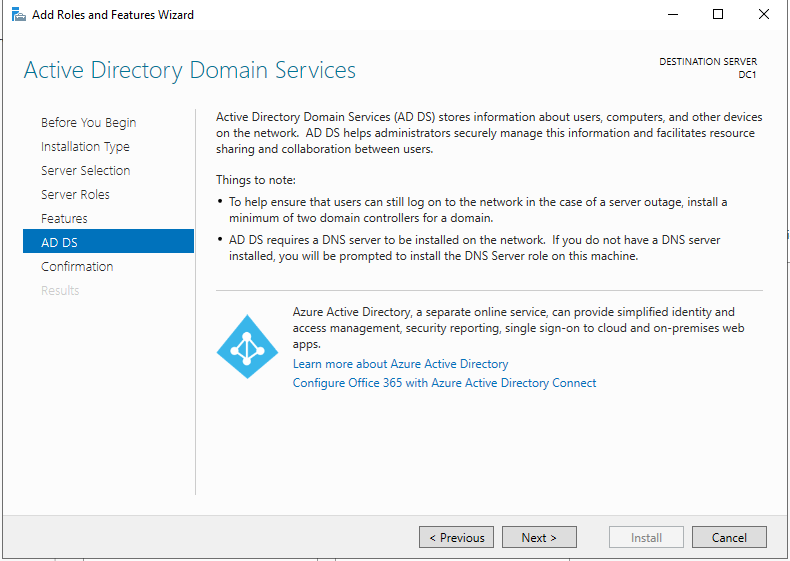
\includegraphics[width=0.7\textwidth]{image/Gui/ADDC/8.png}
			\caption{Cửa sổ Active Directory Domain}
		\end{figure}
		\item Xuất hiện cửa sổ Confirm Installation Selections, chọn \\Server Selection > Next.
		\begin{figure}[htp]
			\centering
			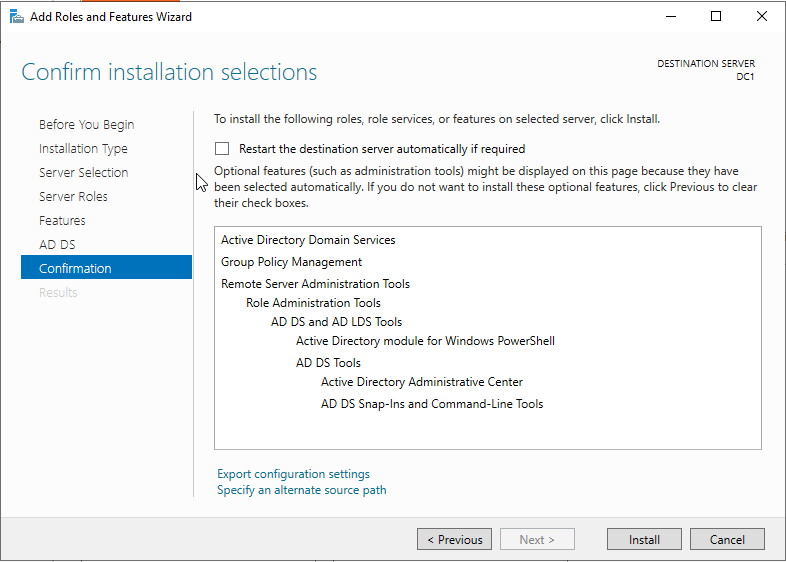
\includegraphics[width=0.7\textwidth]{image/Gui/ADDC/9.png}
			\caption{Cửa sổ Confirm Installation Selections}
		\end{figure}
		\newpage\item Sau khi cài đặt thành công, chọn Promote this server to a domain controller.
		\begin{figure}[htp]
			\centering
			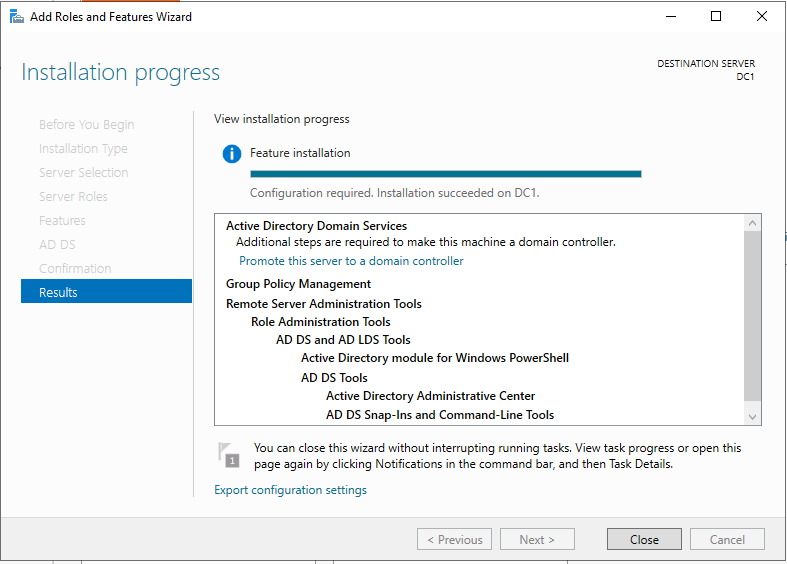
\includegraphics[width=0.7\textwidth]{image/Gui/ADDC/10.png}
			\caption{Cửa sổ cài đặt thành công}
		\end{figure}
		\item Xuất hiện cửa sổ Deployment Configuration, chọn Add a new forest > Nhập root domain name \textbf{“labtdtu.com”} > Next.
		\begin{figure}[htp]
			\centering
			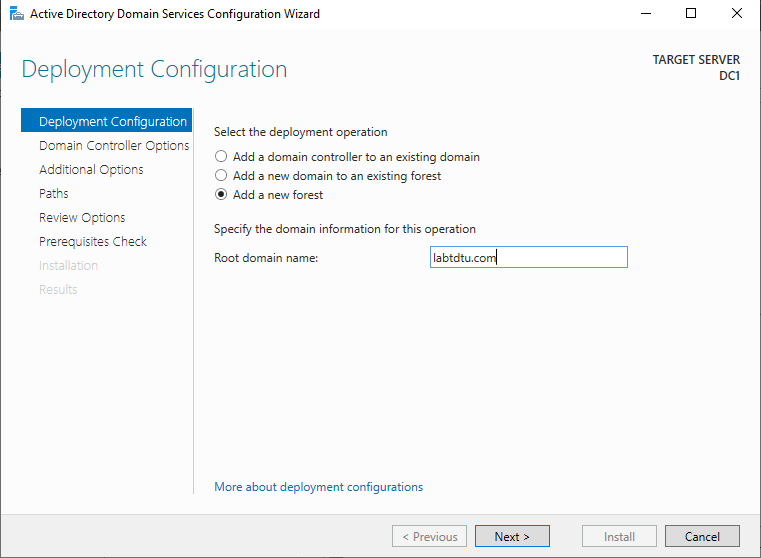
\includegraphics[width=0.7\textwidth]{image/Gui/ADDC/11.png}
			\caption{Cửa sổ Deployment Configuration}
		\end{figure}
		\newpage
		\item Xuất hiện cửa sổ Domain Controller Options, nhập password là \textbf{P@ssw0rd} > Next.
		\begin{figure}[htp]
			\centering
			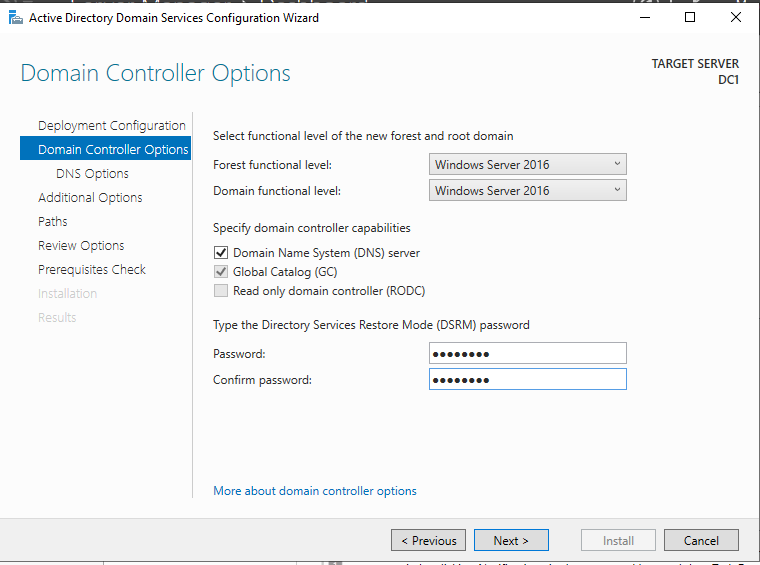
\includegraphics[width=0.7\textwidth]{image/Gui/ADDC/12.png}
			\caption{Cửa sổ Domain Controller Options}
		\end{figure}
		\item Xuất hiện cửa sổ DNS Options, chọn Next.
		\begin{figure}[htp]
			\centering
			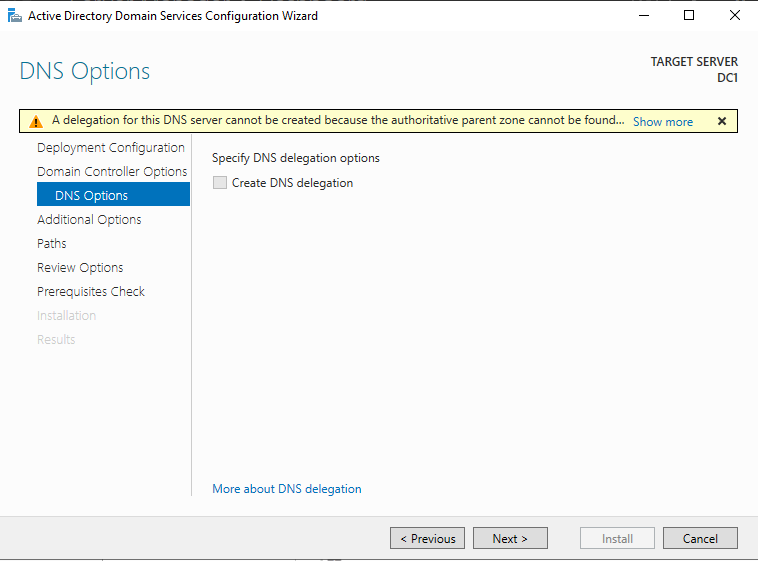
\includegraphics[width=0.67\textwidth]{image/Gui/ADDC/13.png}
			\caption{Cửa sổ DNS Options}
		\end{figure}
		\newpage
		\item Xuất hiện cửa sổ Additional Options > Next
		\begin{figure}[htp]
			\centering
			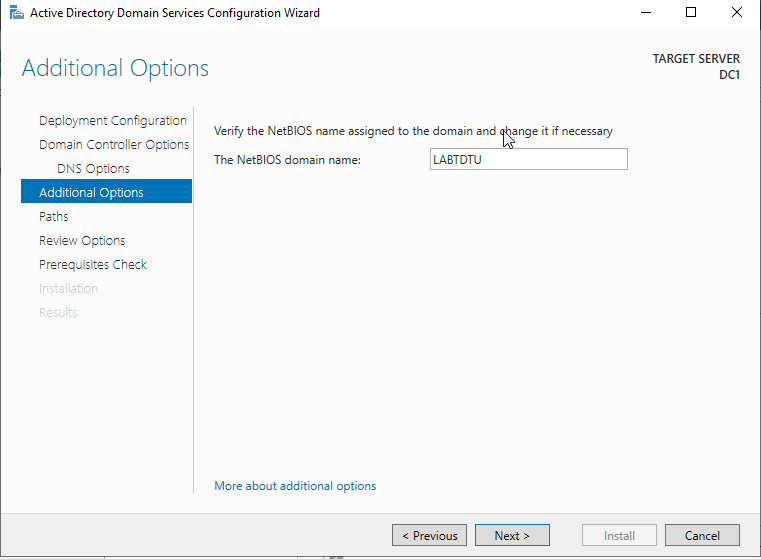
\includegraphics[width=0.7\textwidth]{image/Gui/ADDC/14.png}
			\caption{Cửa sổ Additional Options}
		\end{figure}
		\item Xuất hiện cửa sổ Paths > Next.
		\begin{figure}[htp]
			\centering
			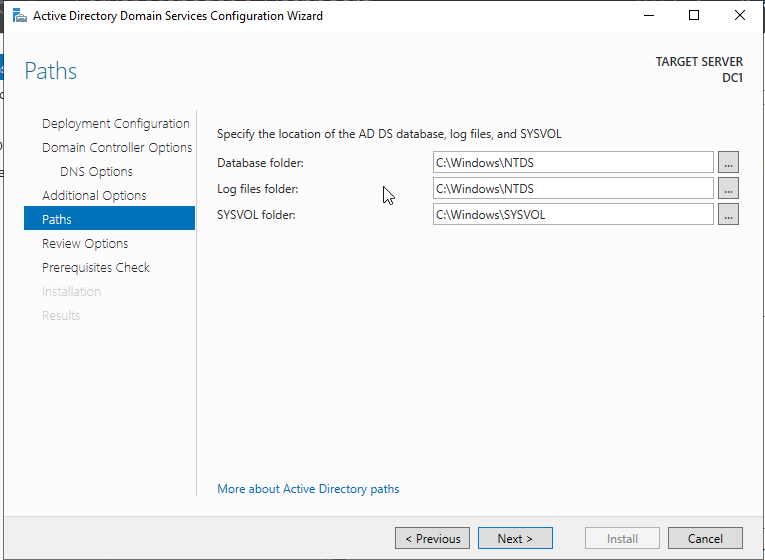
\includegraphics[width=0.7\textwidth]{image/Gui/ADDC/15.png}
			\caption{Cửa sổ Paths}
		\end{figure}
		\newpage
		\item Xuất hiện cửa sổ Review Options, sau đó kiểm tra thông tin > Next.
		\begin{figure}[htp]
			\centering
			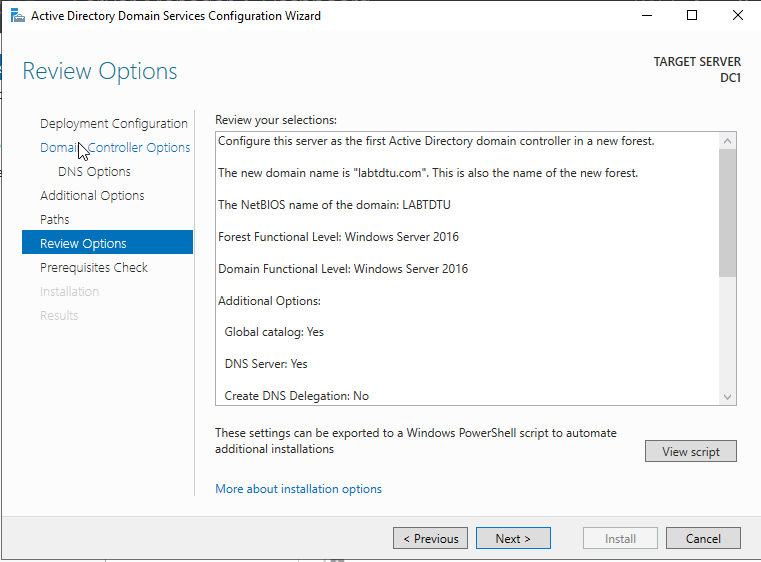
\includegraphics[width=0.7\textwidth]{image/Gui/ADDC/16.png}
			\caption{Cửa sổ Review Options}
		\end{figure}
		\item Xuất hiện cửa sổ Prerequisites Check, chọn Install.
		\begin{figure}[htp]
			\centering
			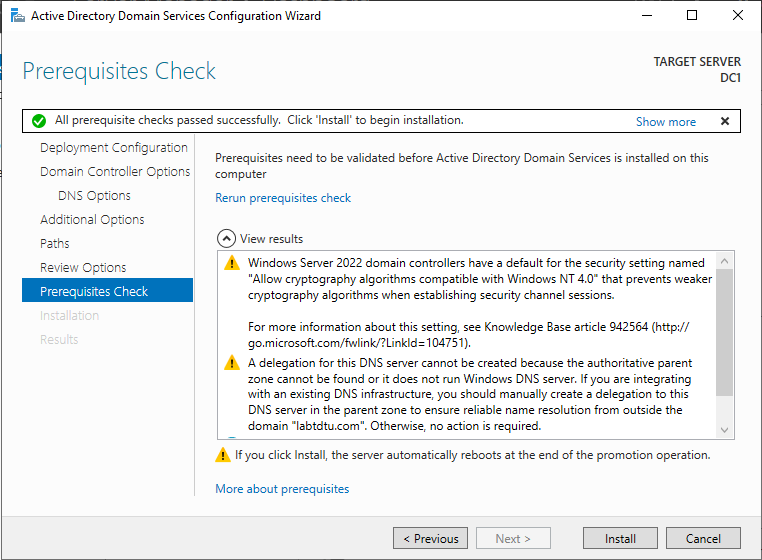
\includegraphics[width=0.7\textwidth]{image/Gui/ADDC/17.png}
			\caption{Cửa sổ Prerequisites Check}
		\end{figure}
		\newpage
		\item Xuất hiện cửa sổ Result là đã cài đặt domain controller thành công.
		\begin{figure}[htp]
			\centering
			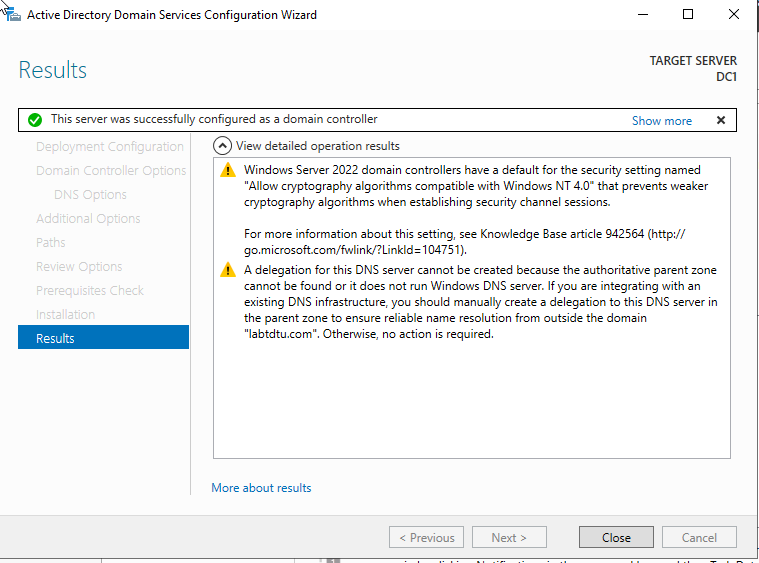
\includegraphics[width=0.7\textwidth]{image/Gui/ADDC/18.png}
			\caption{Cửa sổ Result}
		\end{figure}
	\end{itemize}
	\subsubsection{Join Server vào domain}
	\begin{itemize}
		\item Thiết lập ip cho server như hình sau.
		\begin{figure}[htp]
			\centering
			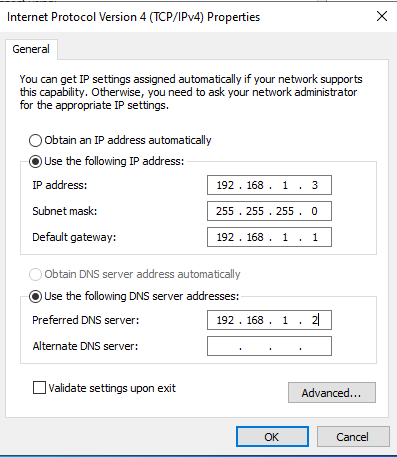
\includegraphics[width=0.45\textwidth]{image/Gui/FIT-WEB/1.png}
			\caption{Thiết lập ip cho server}
		\end{figure}
		\newpage
		\item Từ server ping thành công đến máy domain controller
		\begin{figure}[htp]
			\centering
			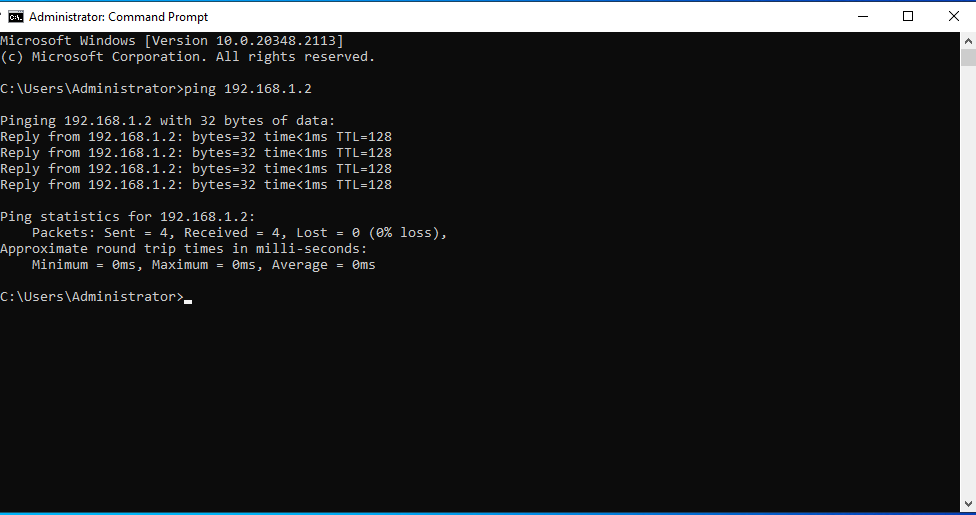
\includegraphics[width=0.7\textwidth]{image/Gui/FIT-WEB/2.png}
			\caption{Ping thành công}
		\end{figure}
		\item Để join vào domain \textbf{labtdtu.com}, vào System Properties > Computer Name > Change
		\begin{figure}[htp]
			\centering
			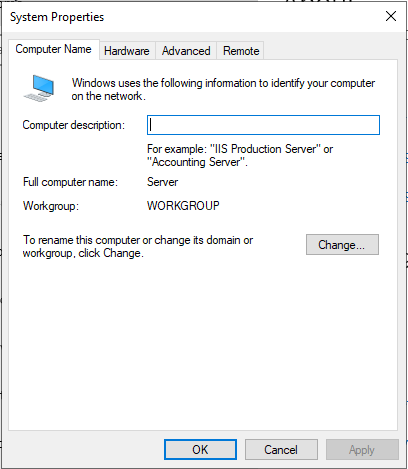
\includegraphics[width=0.58\textwidth]{image/Gui/FIT-WEB/3.png}
			\caption{Join Server vào domain}
		\end{figure}
		\newpage
		\item Member of domain > labtdtu.com
		\begin{figure}[htp]
			\centering
			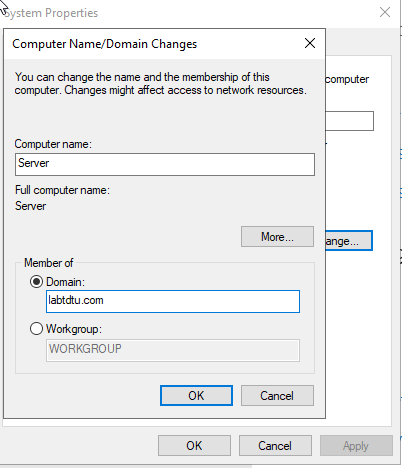
\includegraphics[width=0.56\textwidth]{image/Gui/FIT-WEB/4.png}
			\caption{Nhập domain}
		\end{figure}
		\item Nhập username và password
		\begin{figure}[htp]
			\centering
			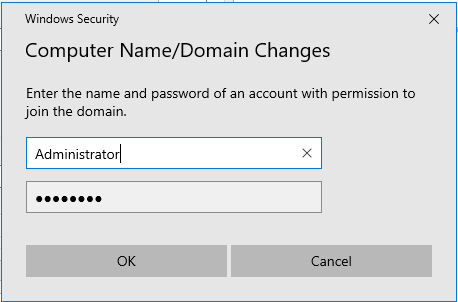
\includegraphics[width=0.56\textwidth]{image/Gui/FIT-WEB/5.png}
			\caption{Xác thực}
		\end{figure}
		\newpage
		\item Join domain thành công
		\begin{figure}[htp]
			\centering
			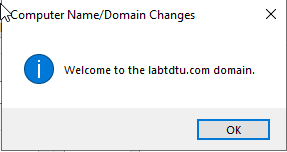
\includegraphics[width=0.5\textwidth]{image/Gui/FIT-WEB/6.png}
			\caption{Join domain thành công}
		\end{figure}
	\end{itemize}
	\subsubsection{Join PC1 vào domain}
	\begin{itemize}
		\item Thiết lập ip cho máy PC1
		\begin{figure}[htp]
			\centering
			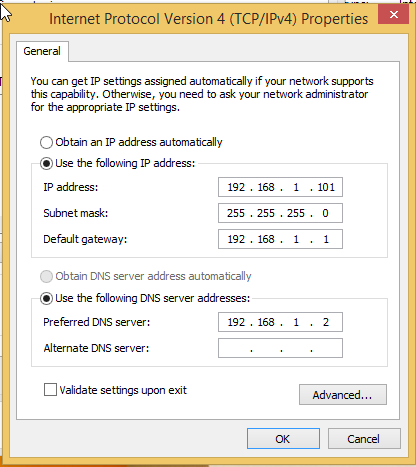
\includegraphics[width=0.6\textwidth]{image/Gui/FIT-PC/1.png}
			\caption{Thiết lập ip cho PC1}
		\end{figure}
		\newpage\item Để join vào domain \textbf{labtdtu.com}, vào System Properties > Computer Name > Change
		\begin{figure}[htp]
			\centering
			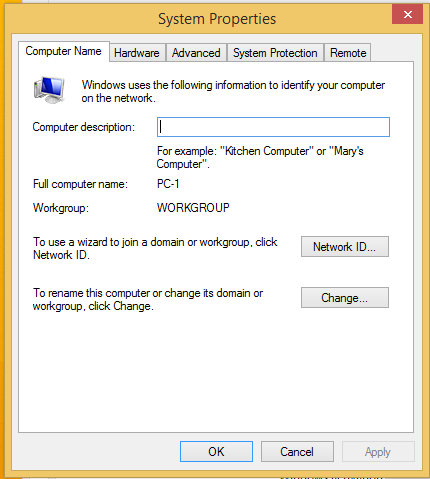
\includegraphics[width=0.45\textwidth]{image/Gui/FIT-PC/2.png}
			\caption{Join PC1 vào domain}
		\end{figure}
		\item Member of domain > labtdtu.com
		\begin{figure}[htp]
			\centering
			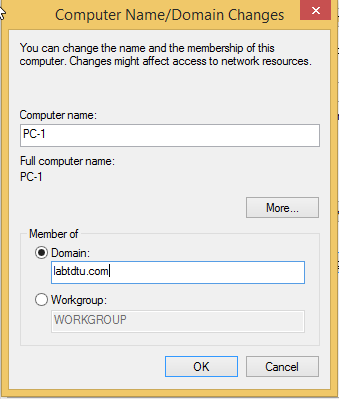
\includegraphics[width=0.45\textwidth]{image/Gui/FIT-PC/3.png}
			\caption{Nhập domain}
		\end{figure}
		\newpage\item Nhập username và password
		\begin{figure}[htp]
			\centering
			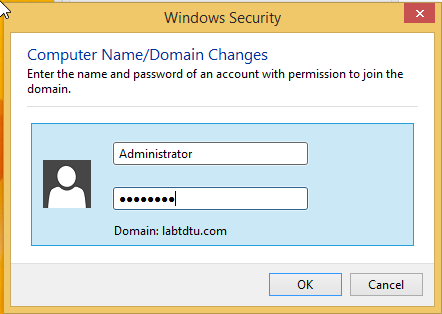
\includegraphics[width=0.7\textwidth]{image/Gui/FIT-PC/4.png}
			\caption{Xác thực}
		\end{figure}
		\item Join domain thành công.
		\begin{figure}[htp]
			\centering
			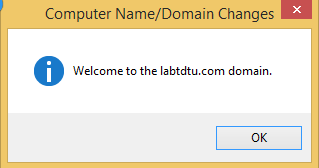
\includegraphics[width=0.7\textwidth]{image/Gui/FIT-PC/5.png}
			\caption{Join domain thành công}
		\end{figure}
	\end{itemize}
	\newpage
	\subsection{Cài Active Directory Certificate Services}
	\begin{itemize}
		\item Trên server, đăng nhập bằng tài khoản \textbf{labtdtu\textbackslash administrator}
		\begin{figure}[htp]
			\centering
			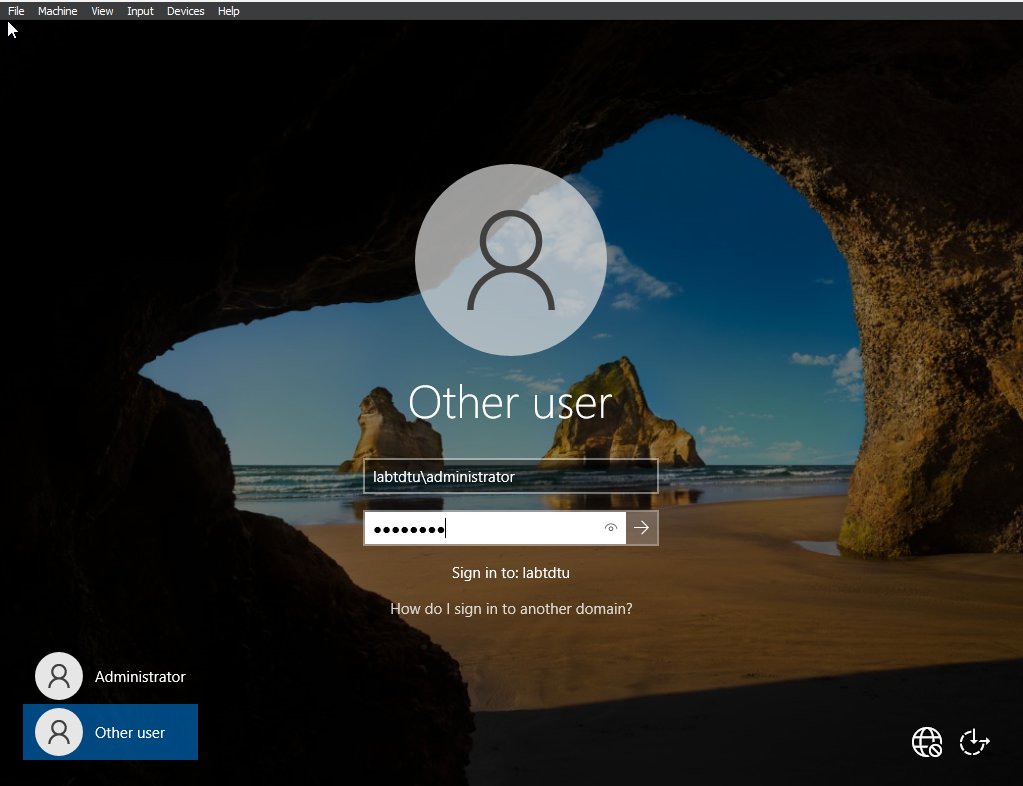
\includegraphics[width=0.6\textwidth]{image/Gui/ADCS/0.png}
			\caption{Đăng nhập bằng tài khoản Administrator}
		\end{figure}
		\item Chọn menu Start > Administrative Tools > Server Manager. Chọn Roles > Add Roles.
		\item Xuất hiện cửa sổ Before You Begin, chọn Next.
		\begin{figure}[htp]
			\centering
			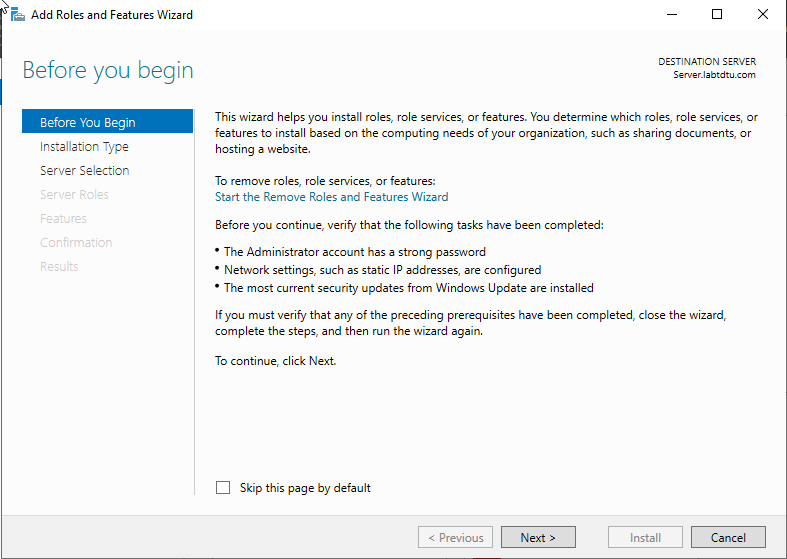
\includegraphics[width=0.7\textwidth]{image/Gui/ADCS/2.png}
			\caption{Cửa sổ Before You Begin}
		\end{figure}
		\newpage
		\item Xuất hiện cửa sổ Select Installation Type, chọn Next.
		\begin{figure}[htp]
			\centering
			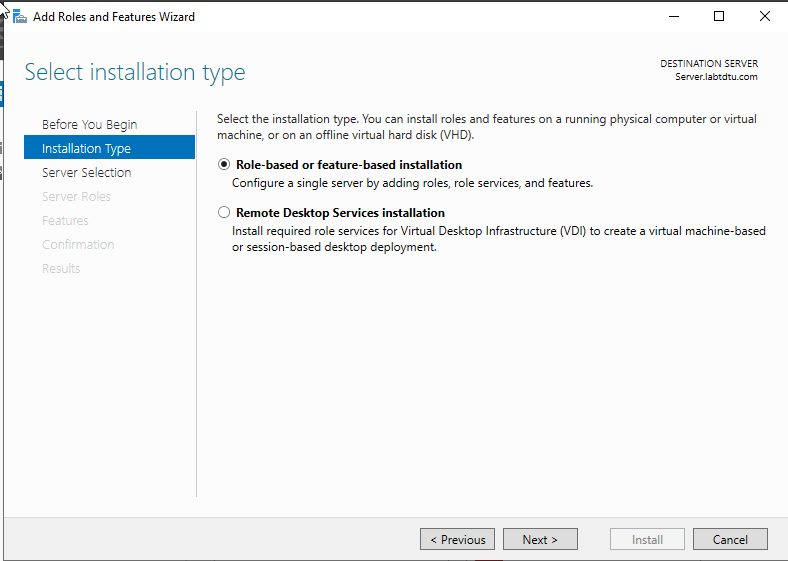
\includegraphics[width=0.7\textwidth]{image/Gui/ADCS/3.png}
			\caption{Cửa sổ Select Installation Type}
		\end{figure}
		\item Xuất hiện cửa sổ Select Destination Server, chọn Next.
		\begin{figure}[htp]
			\centering
			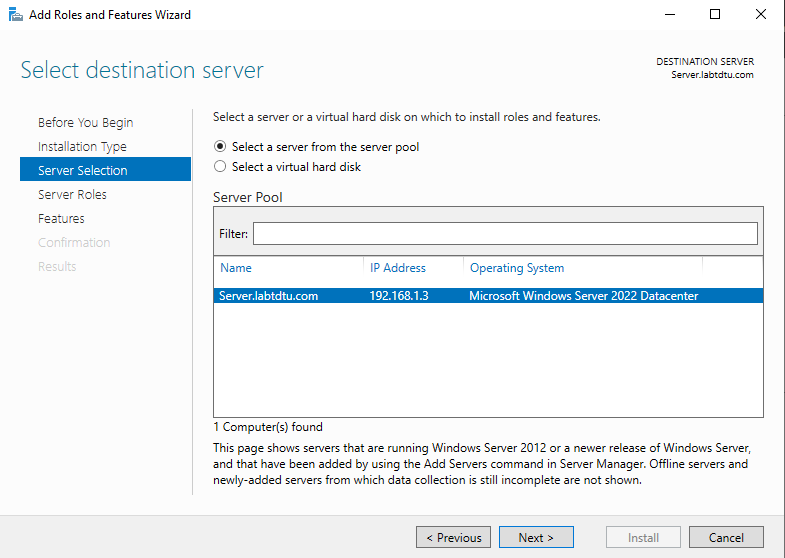
\includegraphics[width=0.7\textwidth]{image/Gui/ADCS/4.png}
			\caption{Cửa sổ Select Destination Server}
		\end{figure}
		\newpage
		\item Xuất hiện cửa sổ Select Server Roles, đánh dấu chọn Active Directory Certificate Service, chọn Next.	
		\begin{figure}[htp]
			\centering
			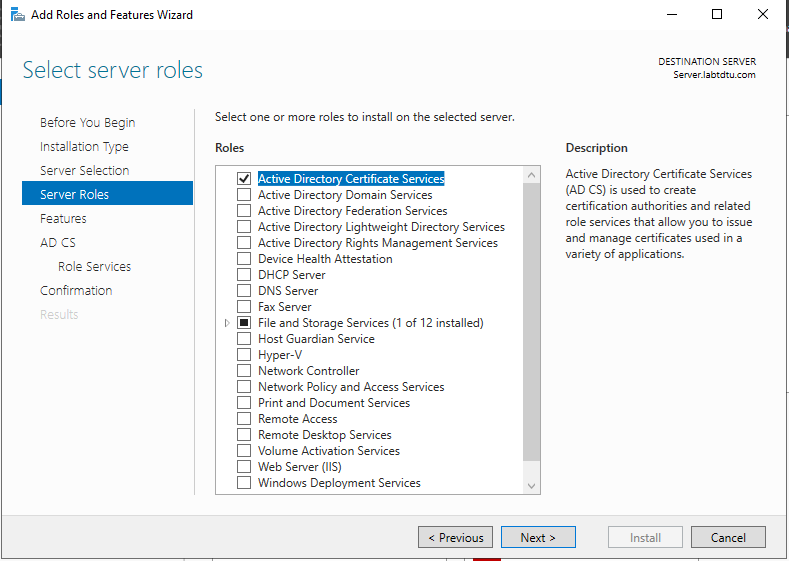
\includegraphics[width=0.7\textwidth]{image/Gui/ADCS/6.png}
			\caption{Cửa sổ Select Server Roles}
		\end{figure}
		\item Các tính năng bổ sung được yêu cầu để thêm AD CS. Nhấp vào nút Add Features.
		\begin{figure}[htp]
			\centering
			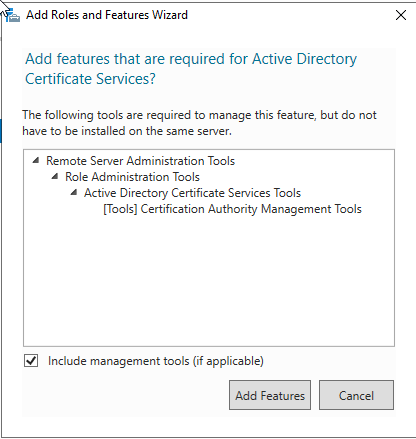
\includegraphics[width=0.5\textwidth]{image/Gui/ADCS/5.png}
			\caption{Cửa sổ các tính năng bổ sung}
		\end{figure}
		\newpage
		\item Xuất hiện cửa sổ Select Features, chọn Next
		\begin{figure}[htp]
			\centering
			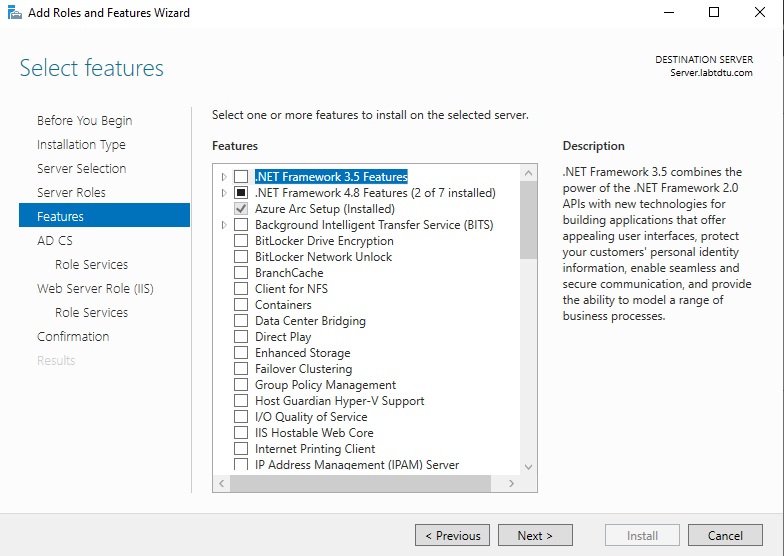
\includegraphics[width=0.7\textwidth]{image/Gui/ADCS/7.png}
			\caption{Cửa sổ Select Features}
		\end{figure}
		\item Xuất hiện cửa sổ Active Directory Certificate Services, chọn Next.
		\begin{figure}[htp]
			\centering
			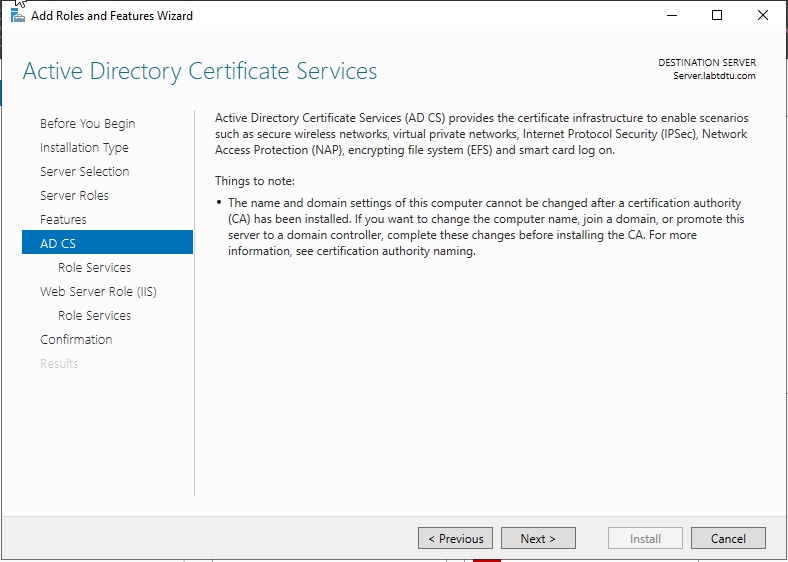
\includegraphics[width=0.7\textwidth]{image/Gui/ADCS/8.png}
			\caption{Cửa sổ Active Directory Certificate Services}
		\end{figure}
		\newpage
		\item Trong cửa sổ Select Role Services, đánh dấu chọn Certificate Authority, Certificate Enrollment Policy Web Service, Certificate Enrollment Web Service, Certification Authority Web Enrollment > Next.
		\begin{figure}[htp]
			\centering
			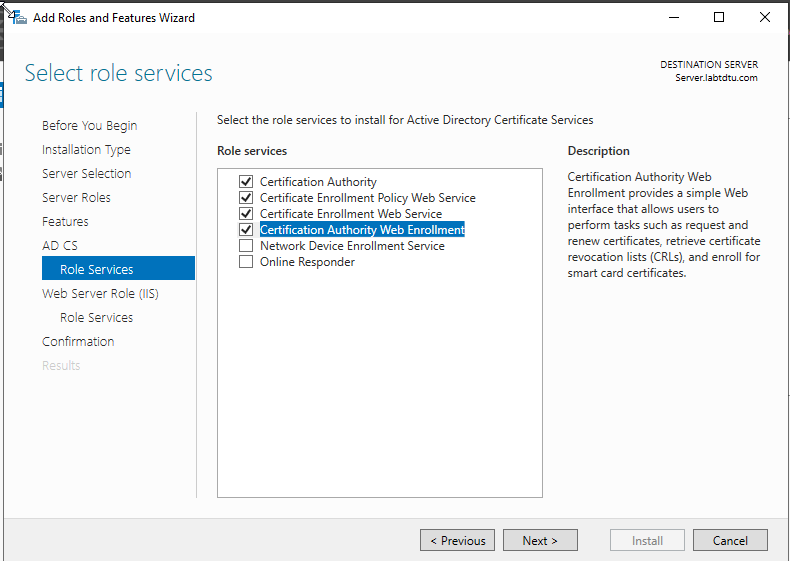
\includegraphics[width=0.7\textwidth]{image/Gui/ADCS/9.png}
			\caption{Cửa sổ Select Role Services}
		\end{figure}
		\item Xuất hiện cửa sổ Web Server (IIS), chọn Next.
		\begin{figure}[htp]
			\centering
			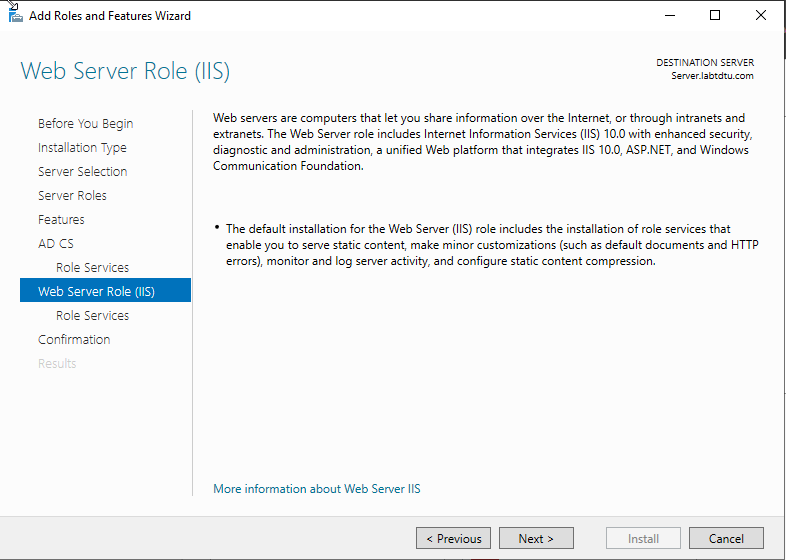
\includegraphics[width=0.7\textwidth]{image/Gui/ADCS/10.png}
			\caption{Cửa sổ Web Server (IIS)}
		\end{figure}
		\newpage
		\item Trong cửa sổ Select Role Services, giữ cấu hình mặc định, chọn Next.
		\begin{figure}[htp]
			\centering
			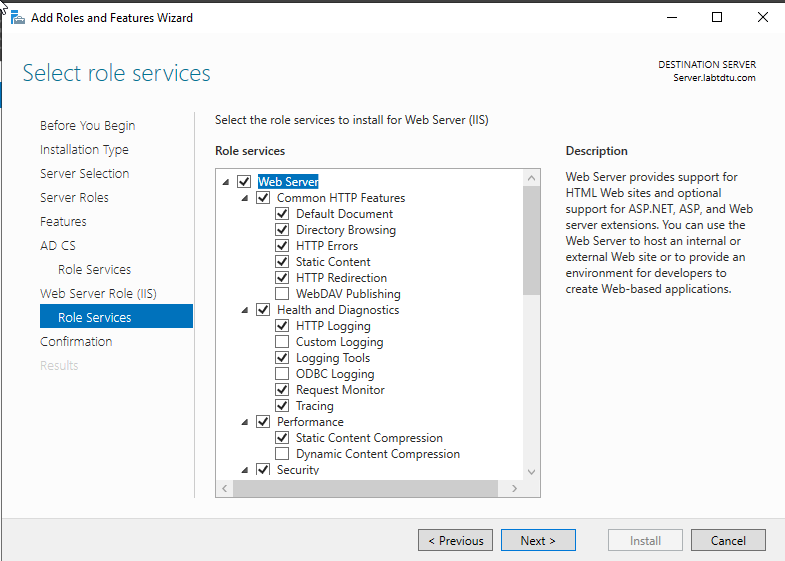
\includegraphics[width=0.7\textwidth]{image/Gui/ADCS/11.png}
			\caption{Cửa sổ Select Role Services}
		\end{figure}
		\item Xuất hiện cửa sổ Confirm Installation Selections, chọn Install.
		\begin{figure}[htp]
			\centering
			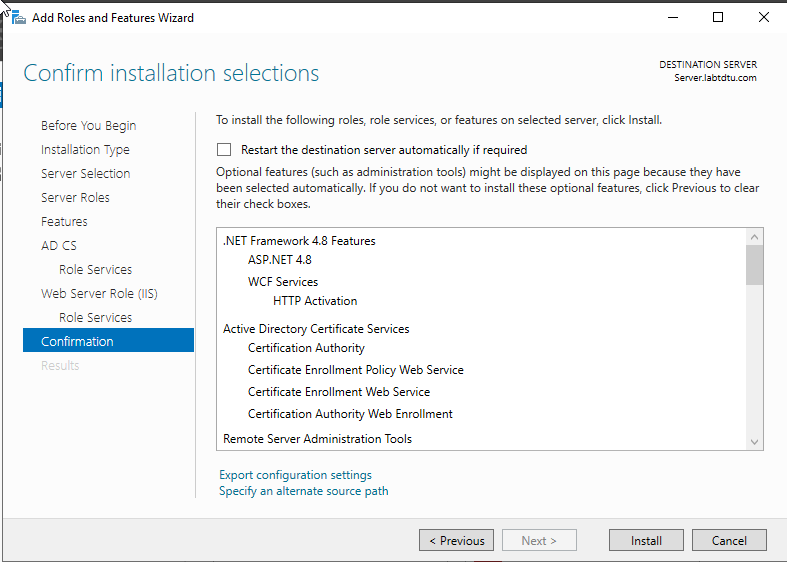
\includegraphics[width=0.7\textwidth]{image/Gui/ADCS/12.png}
			\caption{Cửa sổ Confirm Installation Selections}
		\end{figure}
		\newpage
		\item Sau khi cài đặt thành công, chọn Configure Active Directory Certificate on the destination server.
		\begin{figure}[htp]
			\centering
			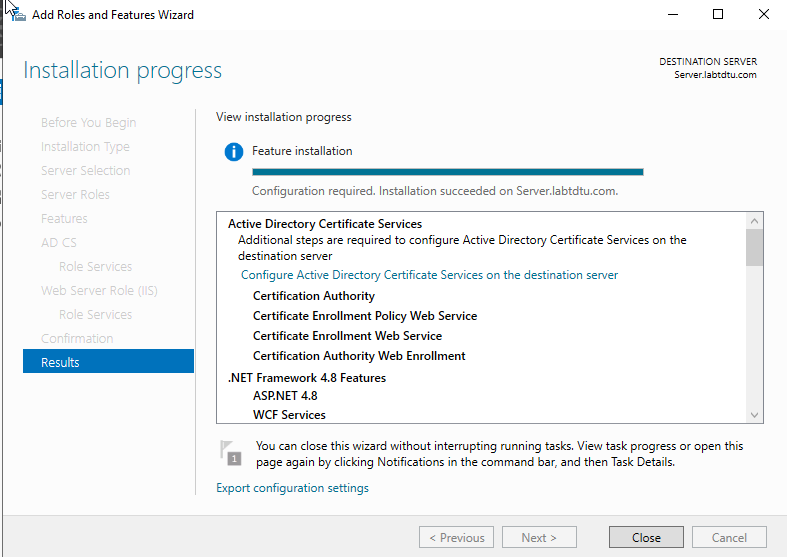
\includegraphics[width=0.7\textwidth]{image/Gui/ADCS/13.png}
			\caption{Cửa sổ cài đặt thành công}
		\end{figure}
		\item Xuất hiện cửa sổ Credentials, chọn Next.
		\begin{figure}[htp]
			\centering
			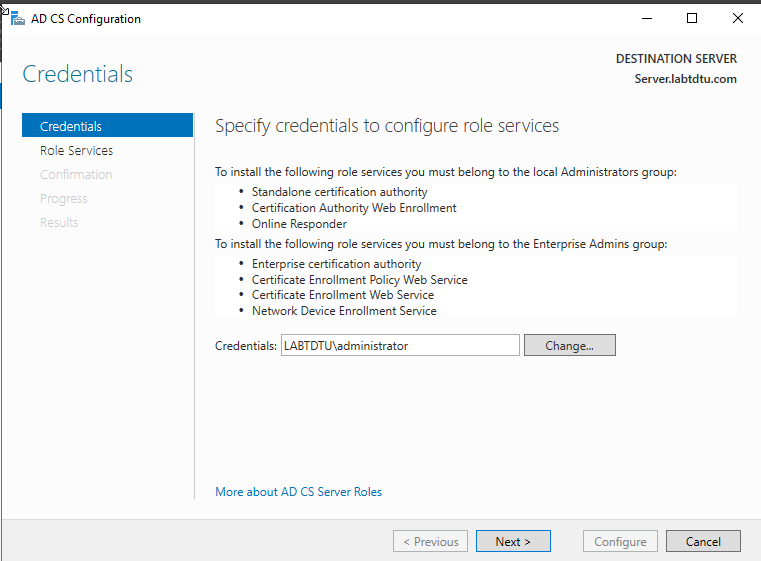
\includegraphics[width=0.7\textwidth]{image/Gui/ADCS/14.png}
			\caption{Cửa sổ Credentials}
		\end{figure}
		\newpage
		\item Xuất hiện cửa sổ Role Services, chọn Certification Authority > Next.
		\begin{figure}[htp]
			\centering
			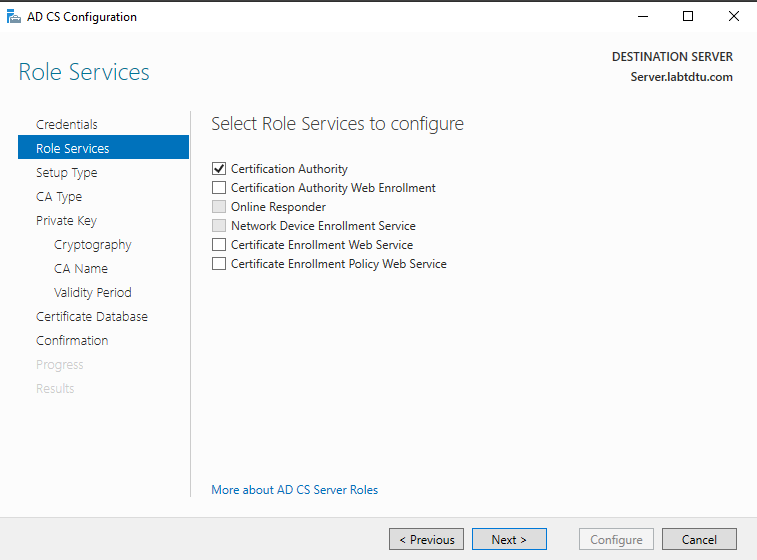
\includegraphics[width=0.7\textwidth]{image/Gui/ADCS/15.png}
			\caption{Cửa sổ Role Services}
		\end{figure}
		\item Xuất hiện cửa sổ Setup Type, chọn Enterprise CA > Next.
		\begin{figure}[htp]
			\centering
			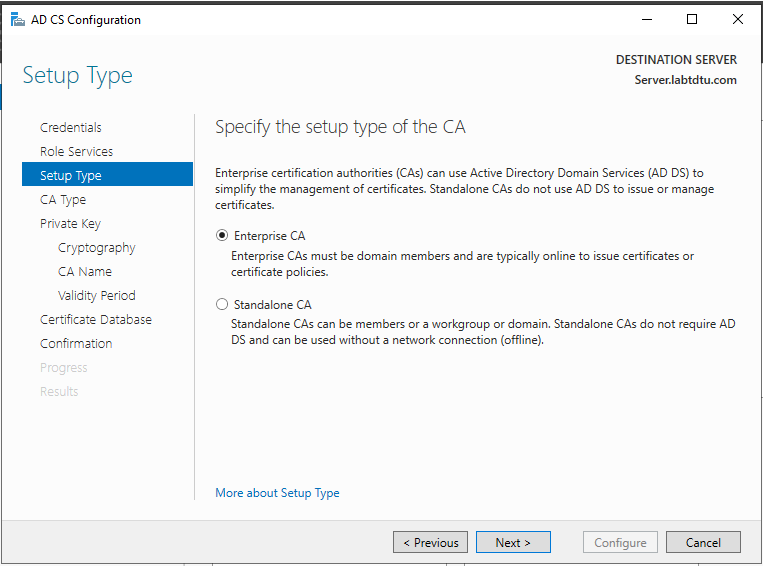
\includegraphics[width=0.7\textwidth]{image/Gui/ADCS/16.png}
			\caption{Cửa sổ Setup Type}
		\end{figure}
		\newpage
		\item Xuất hiện cửa sổ CA Type, do đây là CA đầu tiên nên ta chọn Root CA > Next.
		\begin{figure}[htp]
			\centering
			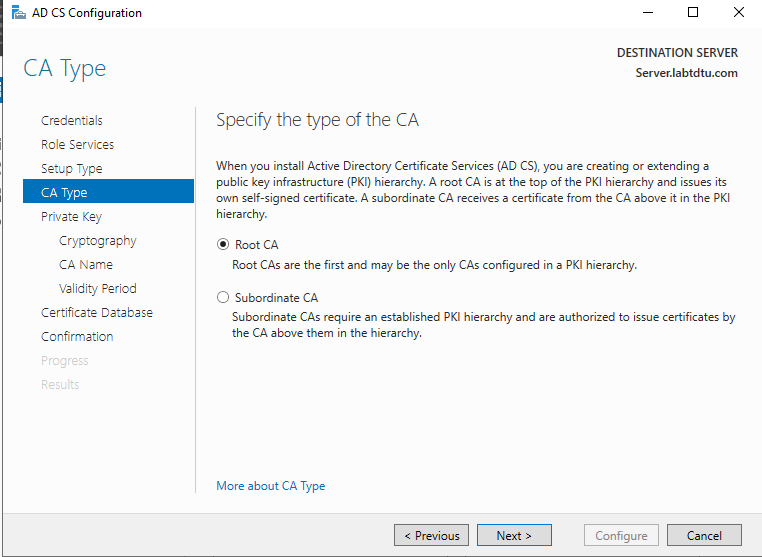
\includegraphics[width=0.7\textwidth]{image/Gui/ADCS/17.png}
			\caption{Cửa sổ CA Type}
		\end{figure}
		\item Xuất hiện cửa sổ Private Key, chọn Create a new private key > Next.
		\begin{figure}[htp]
			\centering
			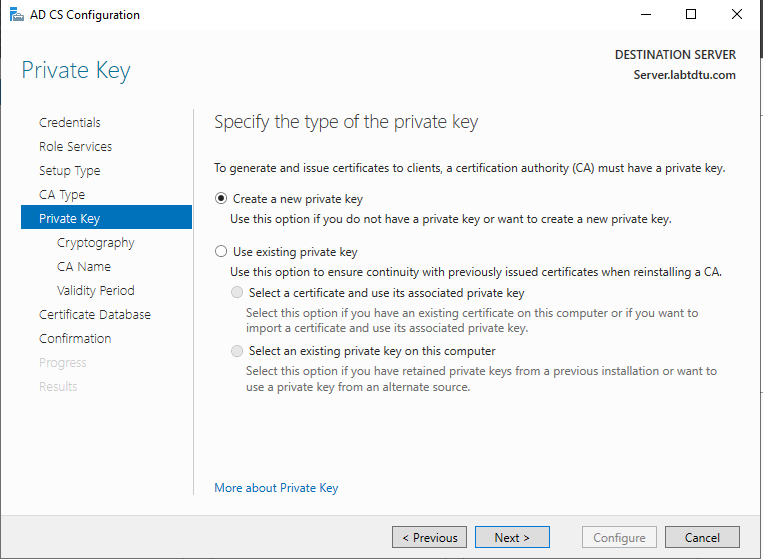
\includegraphics[width=0.7\textwidth]{image/Gui/ADCS/18.png}
			\caption{Cửa sổ Private Key}
		\end{figure}
		\newpage
		\item Trong cửa sổ Cryptography For CA, chọn Next.
		\begin{figure}[htp]
			\centering
			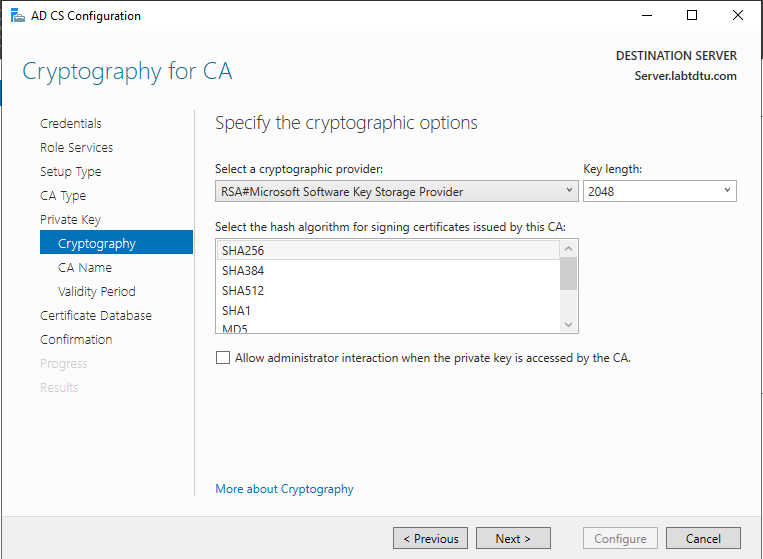
\includegraphics[width=0.7\textwidth]{image/Gui/ADCS/19.png}
			\caption{Cửa sổ Cryptography For CA}
		\end{figure}
		\item Trong cửa sổ CA Name, đặt tên cho CA, ở đây để tên mặc định là labtdtu-SERVER-CA > Next.
		\begin{figure}[htp]
			\centering
			\includegraphics[width=0.7\textwidth]{image/Gui/ADCS/20.png}
			\caption{Cửa sổ CA Name}
		\end{figure}
		\newpage
		\item Trong cửa sổ Validity Period, chọn Next.
		\begin{figure}[htp]
			\centering
			\includegraphics[width=0.67\textwidth]{image/Gui/ADCS/21.png}
			\caption{Cửa sổ Validity Period}
		\end{figure}
		\item Tiếp tục cài đặt 3 role còn lại gồm:
		\begin{itemize} 
			\item Certificate Authority Web Enrollment
			\item Certificate Enrollment Web Service
			\item Certificate Enrollment Policy Web Service
		\end{itemize}
		\begin{figure}[htp]
			\centering
			\includegraphics[width=0.67\textwidth]{image/Gui/ADCS/22.png}
			\caption{Cửa sổ các role còn lại cần cài đặt}
		\end{figure}
		\newpage
		\item Sau khi cài xong 3 role như trên, xuất hiện cửa sổ CA For CES, chọn Next.
		\begin{figure}[htp]
			\centering
			\includegraphics[width=0.7\textwidth]{image/Gui/ADCS/23.png}
			\caption{Cửa sổ CA For CES}
		\end{figure}
		\item Xuất hiện cửa sổ Authentication Type For CES, chọn Next.
		\begin{figure}[htp]
			\centering
			\includegraphics[width=0.7\textwidth]{image/Gui/ADCS/24.png}
			\caption{Cửa sổ Authentication Type For CES}
		\end{figure}
		\newpage
		\item Xuất hiện cửa sổ Service Account For CES, chọn Use the built-in application pool identity > Next.
		\begin{figure}[htp]
			\centering
			\includegraphics[width=0.7\textwidth]{image/Gui/ADCS/25.png}
			\caption{Cửa sổ Service Account For CES}
		\end{figure}
		\item Xuất hiện cửa sổ Authentication Type For CEP, chọn Next.
		\begin{figure}[htp]
			\centering
			\includegraphics[width=0.7\textwidth]{image/Gui/ADCS/26.png}
			\caption{Cửa sổ Authentication Type For CEP}
		\end{figure}
		\newpage
		\item Xuất hiện cửa sổ Server Certificate, chọn chứng chỉ > Next.
		\begin{figure}[htp]
			\centering
			\includegraphics[width=0.6\textwidth]{image/Gui/ADCS/27.png}
			\caption{Cửa sổ Server Certificate}
		\end{figure}
		\item Cài đặt tương tự tự như trên cho máy DC (Domain Controller)
		\subsubsection{Xin SSL Certificate cho Web Server} 
		\item Trên máy DC1, mở Internet Information Services (IIS) Manage từ Administrative Tools. Chọn DC1, trong cửa sổ giữa chọn Server Certificates.
		\begin{figure}[htp]
			\centering
			\includegraphics[width=0.6\textwidth]{image/Gui/SSL/1.png}
			\caption{Xuất hiện cửa sổ DC1 Home}
		\end{figure}
		\newpage
		\item Trong phần Action, chọn Create Certificate Request…
		\begin{figure}[htp]
			\centering
			\includegraphics[width=0.7\textwidth]{image/Gui/SSL/2.png}
			\caption{Xuất hiện Server Certificates}
		\end{figure}
		\item Trong cửa sổ Distinguished Name Properties, nhập thông tin như sau và chọn Next.
		\begin{figure}[htp]
			\centering
			\includegraphics[width=0.7\textwidth]{image/Gui/SSL/3.png}
			\caption{Cửa sổ Distinguished Name Properties}
		\end{figure}
		\newpage
		\item Trong cửa sổ Cryptographic Service Provider Properties, giữ cấu hình mặc định, chọn Next. 
		\begin{figure}[htp]
			\centering
			\includegraphics[width=0.65\textwidth]{image/Gui/SSL/4.png}
			\caption{Cửa sổ Cryptographic Service Provider Properties}
		\end{figure}
		\item Trong cửa sổ File Name nhập đường dẫn \\\textbf{C:\textbackslash Users\textbackslash Administrator\textbackslash Desktop\textbackslash certreq.txt} vào ô \\Specify a file name for the certificate request, chọn Finish.
		\begin{figure}[htp]
			\centering
			\includegraphics[width=0.65\textwidth]{image/Gui/SSL/5.png}
			\caption{Cửa sổ File Name}
		\end{figure}
		\newpage
		\item Trên máy Server, mở Internet Information Services (IIS) Manage từ Administrative Tools. Chọn SERVER > Sites > Default Web Site > CertSrv		\begin{figure}[htp]
			\centering
			\includegraphics[width=0.7\textwidth]{image/Gui/SSL/6.png}
			\caption{Xuất hiện cửa sổ \textbackslash CertSrc Home}
		\end{figure}
		\item Trên máy DC1, mở trình duyệt Internet Explorer và truy cập địa chỉ \textbf{http://192.168.1.3/certsrv}
		\begin{figure}[htp]
			\centering
			\includegraphics[width=0.7\textwidth]{image/Gui/SSL/7.png}
			\caption{Cửa sổ trình duyệt truy cập website}
		\end{figure}
		\newpage
		\item Nhập username và password
		\begin{figure}[htp]
			\centering
			\includegraphics[width=0.65\textwidth]{image/Gui/SSL/8.png}
			\caption{Cửa sổ xác thực}
		\end{figure}
		\item Trong cửa sổ Welcome, chọn Request a certificate
		\begin{figure}[htp]
			\centering
			\includegraphics[width=0.65\textwidth]{image/Gui/SSL/9.png}
			\caption{Cửa sổ Welcome}
		\end{figure}
		\newpage
		\item Trong cửa sổ Request Certificate, chọn advanced certificate request.
		\begin{figure}[htp]
			\centering
			\includegraphics[width=0.65\textwidth]{image/Gui/SSL/10.png}
			\caption{Cửa sổ Request Certificate}
		\end{figure}
		\item Trong cửa sổ Advanced Certificate Request, chọn Submit a certificate request by using a base-64-encoded CMC or PKCS \#10 file, or submit a renewal request by using a base-64-encoded PKCS \#7 file.
		\begin{figure}[htp]
			\centering
			\includegraphics[width=0.65\textwidth]{image/Gui/SSL/11.png}
			\caption{Cửa sổ Advanced Certificate Request}
		\end{figure}
		\newpage
		\item Trong cửa sổ Submit a Certificate Request or Renewal Request, dán nội dung của file certreq.txt vào ô Saved Request, chọn Submit.
		\begin{figure}[htp]
			\centering
			\includegraphics[width=0.65\textwidth]{image/Gui/SSL/12.png}
			\caption{Cửa sổ Submit a Certificate Request or Renewal Request}
		\end{figure}
		\item Sau khi Submit thành công thì xuất hiện cửa sổ Cetificate Issed, chọn Download certificate.
		\begin{figure}[htp]
			\centering
			\includegraphics[width=0.7\textwidth]{image/Gui/SSL/13.png}
			\caption{Cửa sổ Cetificate Issed}
		\end{figure}
		\newpage
		\item Trên máy DC1, quay trở lại Internet Information Services (IIS) Manage từ Administrative Tool. Chọn DC1, trong cửa sổ giữa chọn Server Certificate. Trong phần Action chọn Complete Certificate Request...
		\begin{figure}[htp]
			\centering
			\includegraphics[width=0.6\textwidth]{image/Gui/SSL/14.png}
			\caption{Cửa sổ Internet Information Services (IIS) Manage}
		\end{figure}
		\item Trong cửa sổ Specify Certificate Authority Response, chỉ đường dẫn đến \textbf{C:\textbackslash Users\textbackslash Administrator\textbackslash Desktop\textbackslash certnew.cer}. Nhập tên chứng thực webserver là certificate vào ô Friendly name > chọn Web Hosting ở mục Select a ceftificate store for the new ceftificate > OK.
		\begin{figure}[htp]
			\centering
			\includegraphics[width=0.6\textwidth]{image/Gui/SSL/15.png}
			\caption{Cửa sổ Specify Certificate Authority Response}
		\end{figure}
		\newpage
		\item Kiểm tra trong phần Server Certificate đã có chứng thực webserver tên là certificate hay chưa. Ở đây certificate đã thành công.
		\begin{figure}[htp]
			\centering
			\includegraphics[width=0.7\textwidth]{image/Gui/SSL/16.png}
			\caption{Cửa sổ Server Certificate}
		\end{figure}
	\end{itemize}
	\subsubsection{Thiết lập tên miền DNS và HTTPS Site}
	\begin{itemize}
		\item \textbf{Thiết lập tên miền DNS:} DNS Manager > DC1 > Forward Lookup Zones > labtdtu.com > Chuột Chuột phải chọn new host > Điền ip address là ip web server
		\begin{figure}[htp]
			\centering
			\includegraphics[width=0.7\textwidth]{image/Gui/DNS.png}
			\caption{Cửa sổ thiết lập tên miền DNS}
		\end{figure}
		\newpage
		\item \textbf{Thiết lập HTTPS Site}
		\begin{itemize}
			\item Internet Information Services Manager > DC1-Sites > Default Website > Bindings > Add
			\begin{figure}[htp]
				\centering
				\includegraphics[width=0.65\textwidth]{image/Gui/Https01.png}
				\caption{Cửa sổ thiết lập HTTPS Site}
			\end{figure}
			\item Type->https->SSL certificate->Chọn certificate đã lưu lúc nãy->OK
			\begin{figure}[htp]
				\centering
				\includegraphics[width=0.65\textwidth]{image/Gui/Https02.png}
				\caption{Cửa sổ}
			\end{figure}
		\end{itemize}
	\end{itemize}
	\newpage
	\subsection{Kiểm tra}
	Trên máy PC1, mở trình duyệt Internet Explorer và truy cập:
	\begin{itemize}
		\item Địa chỉ website: \texttt{https//www.labtdtu.com}
		\begin{figure}[htp]
			\centering
			\includegraphics[width=0.7\textwidth]{image/Gui/Test/1.png}
			\caption{Khi truy cập địa chỉ website: https//www.labtdtu.com}
		\end{figure}
		\item Địa chỉ website: \textbf{http//www.labtdtu.com}
		\begin{figure}[htp]
			\centering
			\includegraphics[width=0.7\textwidth]{image/Gui/Test/2.png}
			\caption{Khi truy cập địa chỉ website: http//www.labtdtu.com}
		\end{figure}
	\end{itemize}
	\newpage
	\section{Thực hành trên PowerShell}
	\subsection{Cài đặt Active Directory Domain Controller}
	\begin{itemize}
		\item Trên máy FIT-DC, cấu hình địa chỉ IP
		\begin{figure}[htp]
			\centering
			\includegraphics[width=0.85\textwidth]{image/PowerShell/ADDC/1.png}
			\caption{Cấu hình địa chỉ IP}
		\end{figure}
		\item Kiểm tra cấu hình địa chỉ IP
		\begin{figure}[h]
			\centering
			\includegraphics[width=0.85\textwidth]{image/PowerShell/ADDC/2.png}
			\caption{Kiểm tra địa chỉ IP}
		\end{figure}
		\newpage
		\item Cài đặt \textbf{Active Directory Domain Controller}
		\begin{figure}[htp]
			\centering
			\includegraphics[width=0.85\textwidth]{image/PowerShell/ADDC/3.png}
			\caption{Cài đặt AD DS}
		\end{figure}
		\item Tạo 1 forest  \textbf{labtdtu.com} mới.
		\begin{figure}[htp]
			\centering
			\includegraphics[width=0.85\textwidth]{image/PowerShell/ADDC/4.png}
			\caption{Tạo forest labtdtu com}
		\end{figure}
		\newpage
		\item Kiểm tra xem máy FIT-DC đã trở thành một Domain Controller hay chưa.
		\begin{figure}[htp]
			\centering
			\includegraphics[width=0.85\textwidth]{image/PowerShell/ADDC/5.png}
			\caption{Kiểm tra đã nâng cấp lên DC}
		\end{figure}
		\item Đổi tên server thành FIT-DC.
		\begin{figure}[htp]
			\centering
			\includegraphics[width=0.85\textwidth]{image/PowerShell/ADDC/6.png}
			\caption{Đổi tên cho máy server}
		\end{figure}
		\newpage
		\item Sau khi reset, DNS lúc này thành \texttt{127.0.0.1}
		\begin{figure}[htp]
			\centering
			\includegraphics[width=0.85\textwidth]{image/PowerShell/ADDC/7.png}
			\caption{Kiểm tra lại địa chỉ IP}
		\end{figure}
		\item Cấu hình lại DNS.
		\begin{figure}[htp]
			\centering
			\includegraphics[width=0.85\textwidth]{image/PowerShell/ADDC/8.png}
			\caption{Cấu hình lại DNS}
		\end{figure}
		\newpage
	\end{itemize}
	\subsubsection{Join FIT-WEB vào domain}
	\begin{itemize}
		\item Trên máy Fit-DC, thêm bản ghi cho \textbf{www.labtdtu.com} với địa chỉ \textbf{192.168.1.3}
		\begin{figure}[htp]
			\centering
			\includegraphics[width=0.85\textwidth]{image/PowerShell/FIT-WEB/5.png}
			\caption{Thêm và kiểm tra bản ghi cho website}
		\end{figure}
		\item Trên máy FIT-WEB, cấu hình địa chỉ IP.
		\begin{figure}[htp]
			\centering
			\includegraphics[width=0.85\textwidth]{image/PowerShell/FIT-WEB/1.png}
			\caption{Cài đạt địa chỉ IP}
		\end{figure}
		\newpage
		\item Kiểm tra cấu hình IP.
		\begin{figure}[htp]
			\centering
			\includegraphics[width=0.85\textwidth]{image/PowerShell/FIT-WEB/2.png}
			\caption{Kiểm tra địa chỉ IP}
		\end{figure}
		\item Đổi tên sang FIT-WEB
		\begin{figure}[htp]
			\centering
			\includegraphics[width=0.85\textwidth]{image/PowerShell/FIT-WEB/3.png}
			\caption{Đổi tên thành FIT-WEB}
		\end{figure}
		\newpage
		\item Join FIT-WEB vào domain labtdtu.com
		\begin{figure}[htp]
			\centering
			\includegraphics[width=0.85\textwidth]{image/PowerShell/FIT-WEB/4.png}
			\caption{Join vào domain}
		\end{figure}	
	\end{itemize}
	\subsubsection{Join máy FIT-WIN08-01 vào domain}
	\begin{itemize}
		\item Cấu hình địa chỉ IP cho \textbf{FIT-WIN08-01} có địa chỉ ip là 192.168.1.101
		\item Join máy FIT-WIN08-01 vào domain labtdtu.com
		\begin{figure}[htp]
			\centering
			\includegraphics[width=0.85\textwidth]{image/PowerShell/FIT-WIN08-01/1.png}
			\caption{Máy client (192.168.1.101) test join vào domain}
		\end{figure}
		\newpage
		\item Kiểm tra join vào domain thành công hay chưa.
		\begin{figure}[htp]
			\centering
			\includegraphics[width=0.85\textwidth]{image/PowerShell/FIT-WIN08-01/2.png}
			\caption{Kết quả join vào domain}
		\end{figure}
	\end{itemize}
	\subsection{Cài Active Directory Certificate Services role}
	\subsubsection{Cấu hình web server (IIS)}
	\begin{itemize}
		\item Cài đặt cấu hình Web Server bằng lệnh
		\begin{figure}[htp]
			\centering
			\includegraphics[width=0.85\textwidth]{image/PowerShell/IIS1.png}
			\caption{cài đặt IIS}
		\end{figure}
		\newpage
		\item Truy cập thử website http://www.labtdtu.com
		\begin{figure}[htp]
			\centering
			\includegraphics[width=0.85\textwidth]{image/PowerShell/IIS2.png}
			\caption{Truy cập website với http}
		\end{figure}
	\end{itemize}
	\subsubsection{Cấu hình Active Directory Certificate Services}
	\begin{itemize}
		\item Cài đặt \textbf{Active Directory Certificate Services}
		\begin{figure}[htp]
			\centering
			\includegraphics[width=0.85\textwidth]{image/PowerShell/ADCS/1.png}
			\caption{Cài đặt AD CS}
		\end{figure}
		\newpage
		\item Cấu hình \textbf{Active Directory Certificate Services}
		\begin{figure}[htp]
			\centering
			\includegraphics[width=0.85\textwidth]{image/PowerShell/ADCS/2.png}
			\caption{Cấu hình AD CS cài đặt CA}
		\end{figure}
		\item Cài đặt \textbf{CA Web Enrollment}
		\begin{figure}[htp]
			\centering
			\includegraphics[width=0.85\textwidth]{image/PowerShell/ADCS/3.png}
			\caption{Cài đặt CA Web Enrollment}
		\end{figure}
		\newpage
		\item Cài đặt \textbf{Online responder}
		\begin{figure}[htp]
			\centering
			\includegraphics[width=0.85\textwidth]{image/PowerShell/ADCS/4.png}
			\caption{Cài đặt Online responder}
		\end{figure}
		\item Tạo \textbf{Certificate Request}
		\begin{figure}[htp]
			\centering
			\includegraphics[width=0.85\textwidth]{image/PowerShell/ADCS/5.png}
			\caption{Tạo Certificate Request}
		\end{figure}
		\newpage
		\item Truy cập trang  \textbf{http://192.168.1.2/certsrv} > Chọn \textbf{Request a Certificate}
		\begin{figure}[htp]
			\centering
			\includegraphics[width=0.85\textwidth]{image/PowerShell/ADCS/6.png}
			\caption{Truy cập certsrv chọn Request a Certificate}
		\end{figure}
		\item	Chọn \textbf{Submit}
		\begin{figure}[htp]
			\centering
			\includegraphics[width=0.85\textwidth]{image/PowerShell/ADCS/7.png}
			\caption{Submit}
		\end{figure}
		\newpage
		\item Chọn \textbf{Submit a certificate request by using base-64-encoded..} 
		\begin{figure}[htp]
			\centering
			\includegraphics[width=0.85\textwidth]{image/PowerShell/ADCS/8.png}
			\caption{Submit a certificate request by using base-64-encoded…}
		\end{figure}
		\item Copy nội dung \textbf{CSR} và paste vào và chọn template webserver.
		\begin{figure}[htp]
			\centering
			\includegraphics[width=0.85\textwidth]{image/PowerShell/ADCS/9.png}
			\caption{Copy nội dung CSR và paste vào và chọn template webserver}
		\end{figure}
		\newpage
		\item Submit thành công, chọn \textbf{Download certificate} tải chứng chỉ về máy. 
		\begin{figure}[htp]
			\centering
			\includegraphics[width=0.85\textwidth]{image/PowerShell/ADCS/10.png}
			\caption{Download Certificate}
		\end{figure}
		\item Lấy đường dẫn tới file certnew vừa được tải.
		\begin{figure}[htp]
			\centering
			\includegraphics[width=0.85\textwidth]{image/PowerShell/ADCS/11.png}
			\caption{Lấy đường dẫn tới file certnew vừa được tải}
		\end{figure}
		\newpage
		\item Hoàn thành chứng chỉ
		\begin{figure}[htp]
			\centering
			\includegraphics[width=0.85\textwidth]{image/PowerShell/ADCS/12.png}
			\caption{Complete chứng chỉ}
		\end{figure}
		\item Kiểm tra chứng chỉ đã được tạo
		\begin{figure}[htp]
			\centering
			\includegraphics[width=0.85\textwidth]{image/PowerShell/ADCS/13.png}
			\caption{Chứng chỉ đã được tạo}
		\end{figure}
	\end{itemize}
	\newpage
	\subsubsection{Tạo Https cho Website}
	Binding https trên port 443 cho website
	\begin{figure}[htp]
		\centering
		\includegraphics[width=0.85\textwidth]{image/PowerShell/Https.png}
		\caption{Chứng chỉ đã được tạo}
	\end{figure}
	\subsection{Kiểm tra}
	\begin{itemize}
		\item Truy cập website labtdtu.com trên máy FIT-WIN08-01 (Chưa có chứng chỉ)
		\begin{figure}[htp]
			\centering
			\includegraphics[width=0.85\textwidth]{image/PowerShell/Test/1.png}
			\caption{Truy cập website trên máy PC client}
		\end{figure}
		\newpage
		\item Truy cập http://192.168.1.2/certsrv để tải chứng chỉ CA về máy
		\begin{figure}[htp]
			\centering
			\includegraphics[width=0.85\textwidth]{image/PowerShell/Test/2.png}
			\caption{Truy cập để tải CA}
		\end{figure}
		\item Tải chứng chỉ 
		\begin{figure}[htp]
			\centering
			\includegraphics[width=0.85\textwidth]{image/PowerShell/Test/3.png}
			\caption{Download CA}
		\end{figure}
		\newpage
		\item Trên IE -> Bánh răng -> Internet Options -> Content -> Certificate
		\begin{figure}[htp]
			\centering
			\includegraphics[width=0.85\textwidth]{image/PowerShell/Test/4.png}
			\caption{Bánh răng - Internet Options - Tab Content - Certificate}
		\end{figure}
		\item Import file vừa tải vào Trusted Root Certification Authorities
		\begin{figure}[htp]
			\centering
			\includegraphics[width=0.85\textwidth]{image/PowerShell/Test/5.png}
			\caption{Import file vừa tải vào Trusted Root Certification Authorities}
		\end{figure}
		\newpage
		\item Import hoàn tất
		\begin{figure}[htp]
			\centering
			\includegraphics[width=0.85\textwidth]{image/PowerShell/Test/6.png}
			\caption{Đã import}
		\end{figure}
		\item Truy cập lại https://www.labtdtu.com
		\begin{figure}[htp]
			\centering
			\includegraphics[width=0.85\textwidth]{image/PowerShell/Test/7.png}
			\caption{Truy cập lại website}
		\end{figure}
	\end{itemize}
	\chapter{Kết luận}
	Sau khi kết thúc bài đồ án cuối kỳ, nhóm 20 đã nắm được những nội dung như sau:
	\begin{itemize}
		\item Hiểu về hoạt động của Active Directory Certificate Services (AD CS)
		\begin{itemize}
			\item Biết cách AD CS tạo và quản lý chứng chỉ số.
			\item Hiểu về quy trình cấp phát chứng chỉ và quy trình xác thực.
			\item Nắm rõ về các thành phần chính của AD CS như Certification Authority (CA), Registration Authority (RA), và Database.
		\end{itemize}
		\item Vận dụng AD CS để bảo mật website
		\begin{itemize}
			\item Biết cách sử dụng AD CS để tạo và quản lý chứng chỉ số SSL/TLS.
			\item Hiểu về ưu điểm của việc sử dụng chứng chỉ SSL/TLS trong bảo mật website, bao gồm cả mức độ bảo mật cao và sự tin cậy từ phía người sử dụng.
			\item Có khả năng triển khai chứng chỉ trong môi trường web server.
		\end{itemize}
		\item Thực hành trên giao diện đồ họa (GUI)
		\begin{itemize}
			\item Biết cách sử dụng giao diện quản lý của AD CS để thực hiện các tác vụ như cấp chứng chỉ.
			\item Có khả năng thực hiện các thao tác quản lý chứng chỉ thông qua giao diện người dùng.
		\end{itemize}
		\item Thực hành bằng PowerShell
		\begin{itemize}
			\item Hiểu cách sử dụng PowerShell để tự động hóa các tác vụ liên quan đến AD CS.
			\item Có khả năng tạo, quản lý, và thực hiện các tác vụ khác liên quan đến chứng chỉ bằng PowerShell.
		\end{itemize}
	\end{itemize}
	Bên cạnh đó, nhóm 20 chưa nắm vững được các kiến thức về tư duy an toàn như là hiểu về các best practices khi triển khai AD CS để đảm bảo tính ổn định và an toàn hay là nắm vững về quản lý khóa và chứng chỉ, cũng như quản lý chuỗi chứng chỉ.
	\begin{thebibliography}{99}
		\bibitem{}Brian Desmond, \textit{Active Directory 5th edition}, 2003
		\bibitem{}Mike F. Robbins, \textit{PowerShell 101}, 2020
		\bibitem{}Microsoft, \textit{Implement and manage Active Directory Certificate Services}
	\end{thebibliography}
\end{document}